\documentclass[a4paper, titlepage]{article}
\renewcommand{\baselinestretch}{1.15}				% line spacing 

% Package list
\usepackage{amsmath}
\usepackage[url=true, 
			backend=biber, 	
			style=ieee,
			sorting=none, 
			hyperref=true]{biblatex}	% remove url visit date and sort references by appearance
\usepackage{hyperref}
\usepackage{xurl}
\usepackage{helvet}									% helvetica font
\usepackage{rotating}
\usepackage{array}
\usepackage{multirow}
\usepackage{xpatch}
\newcolumntype{C}[1]{>{\centering\arraybackslash}p{#1}}

\renewcommand{\thefootnote}{\alph{footnote}}
% Biblatex configuratin
\addbibresource{library.bib}
\DeclareNameAlias{author}{family-given}

% ideas for paper
% add carbon taxes
% add ports as possible sinks
% add eucalyptus
% add electrolysis
% lower urea demand

\begin{document}
\title{Renewable urea production integrated with agricultural residue gasification; a process modeling and
supply-chain hybrid approach}
\author{
	Diego Lopes\\
	\and
	Moisés Teles dos Santos}
\date{01/07/2025}
\maketitle

\begin{abstract}
Nitrogen fertilizers are important energy consumers on the chemical sector and are responsible for considerable GHG
emissions. However, the conventional process is dependent on fossil fuels and the renewable fraction of urea on the
market is negligible. The present work proposes a hybrid model for a renewable urea plant through gasification of
agricultural residues, combining traditional process modeling techniques with an optimization framework. The process
model was applied to 6 biomasses representative of the Brazilian market and 2 operational conditions. The process model
results are fed into a MILP model to evaluate the optimal combination of location, biomass and technological route that
maximizes the NPV of the renewable urea plant. Processing sugarcane straw with air mixed gasification in the state of
São Paulo is proven to be the best combination with current biomass, urea and power prices. Urea demand and 
distribution costs are shown to be a critical factor in the feasibility of the plant, which corroborates the importance
of a hybrid approach in evaluating any biorefinery configuration. 
\end{abstract}

\section{Introduction}

Since 1961, worldwide food supply per capita has raised by 30\%, in large part because of the increase of use of
nitrogen fertilizers to improve agricultural productivity \cite{mbowIPCCSpecialReport2019}. The importance of
fertilizers on agriculture cannot be overstated, with research indicating that half of the world’s population
is sustained by mineral fertilizers. The agricultural sector is also responsible for between 11\% and 15\% of
all greenhouse gas (GHG) emissions worldwide \cite{ifaEstimatingReportingFertilizerRelated2016}, with fertilizers
accounting for 2\% to 3\% of emissions \cite{brentrupCarbonFootprintAnalysis2016}. Production of mineral fertilizers
is dependent on fossil fuels and raw materials, including mineral extraction,
transportation, manufacturing, and power supply. In this scenario, decarbonizing the fertilizer sector is equally
important to the industry’s expansion \cite{ouikhalfanNetZeroEmissionFertilizers2022}, considering the GHG emissions
reduction preconized in the Paris agreement (2015).

The mineral fertilizers divide themselves into three main categories, each one corresponding to the main
macronutrient present in its composition: nitrogen (N), phosphorus (P) and potassium (K). Although none of the
macronutrients can be considered more or less important than the other, nitrogen is the one consumed at higher
volumes, and also the one with the more energetically intensive manufacturing
process \cite{ieaAmmoniaTechnologyRoadmap2021}. Out of all nitrogen fertilizers, urea is the main commercial product,
with ammonia as its obligatory precursor. Ammonia ($NH_3$) is obtained by the synthesis of hydrogen ($H_2$)
and nitrogen $N_2$ through the traditional Haber-Bosch process, responsible for the production of more than 90\% of
worldwide ammonia \cite{applAmmoniaPrinciplesIndustrial1999}. Nitrogen is obtained from the atmosphere,
but hydrogen is traditionally obtained from steam reforming of fossil fuels; 72\% of the worldwide ammonia
production comes from natural gas reforming, while 26\% is obtained from coal gasification. 1\% is produced
through other petroleum derivatives, while the renewable fraction, produced through water electrolysis,
corresponds to less than 1\% \cite{ieaAmmoniaTechnologyRoadmap2021}. Urea, in turn, is produced by the Basarov reaction
using ammonia and carbon dioxide ($CO_2$), with this process being responsible for all commercial urea production
in a large scale \cite{meessenUrea2010}. The $CO_2$ is supplied by the reforming syngas, as both $CO$ and $CO_2$ must
be removed prior to the ammonia synthesis as they are poisons to the commercial catalysts.

Since both processes are energetically intensive, efforts were made throughout the 20\textsuperscript{th} century to
improve its energy efficiency, involving equipment changes, process control and residual heat utilization. With these
efforts, current ammonia production is very close to the theoretical minimum energy consumption
\cite{ieaAmmoniaTechnologyRoadmap2021}.
Considering the small efficiency improvements still possible, a natural future step is to search for sustainable
replacements for the process’ feedstocks and energy usages.

In this scenario, biomass is a promising feedstock replacement. Among the conversion routes, gasification is of special
interest considering that the biomass syngas composition is similar to the fossil fuel syngas obtained in traditional
processes; in that sense the conversion technologies of this syngas into alcohols, hydrocarbons and other chemicals
can be leveraged with significant overlap. Despite that, biorefineries pose additional challenges to the conventional
plants. Given its high volume and low energetic density compared to fossil fuels, the feasibility of all biorefineries
depend heavily on the local availability of biomass inputs and spatial allocation of this biomass
. This demonstrates the need for an integrated approach in biorefinery
modeling that combines technical performance, location, capacity and configuration of the plant
\cite{schroderImprovingBiorefineryPlanning2018}.

\section{Literature Review}

The mathematical modeling of biomass gasification, ammonia, urea and its subprocesses has been the object of multiple
studies. \textcite{baruahModelingBiomassGasification2014} presented a systematic review of  existing techniques to model
biomass gasification systems, categorized by gasifier type, feedstock and parameters studied,
concluding that equilibrium modeling is the most suitable technique for process studies on the influence of fuel and
process parameters, since these models are independent of gasifier's design.
\textcite{gambarottaNonstoichiometricEquilibriumModel2018} and \textcite{azzoneDevelopmentEquilibriumModel2012} developed
equilibrium models for biomass gasification and compared the model’s results against experimental data, predicting the
syngas composition with reasonable accuracy. Gasification models were successfully implemented in commercial process
simulators such as Aspen Plus, in \textcite{hanModelingDowndraftBiomass2017} and
\textcite{ramzanSimulationHybridBiomass2011}

The ammonia synthesis process has also been modeled extensively. The reaction mechanisms and kinetics have been
studied since the 1930s \cite{gillespieThermodynamicTreatmentChemical1930} and the Temkin-Pyzhev formulation is
used to this day in ammonia reactor designs \cite{temkinKineticsAmmoniaSynthesis1940}
\cite{singhSimulationAmmoniaSynthesis1979} \cite{nielsenAmmoniaCatalysisManufacture1995}.
\textcite{florez-orregoProcessSynthesisOptimization2018} has modeled the full fossil fuel process and conducted
exergy analysis and optimization while \textcite{domingosExergyEnvironmentalAnalysis2021} has applied the same model
for ammonia production through black liquor gasification, with promising results reaching negative emissions in
certain scenarios. Ammonia production via other biomasses have also been proposed by
\textcite{florez-orregoComparativeExergyEconomic2019} and \textcite{tunaTechnoeconomicAssessmentNonfossil2014}, with
both studies identifying substantial environmental benefits in using biomass as a feedstock, despite a lower energy
efficiency in the process.

The urea process is also studied since the start of the 20\textsuperscript{th} century, with early works on the
urea synthesis published by \textcite{frejacquesBasesTheoriquesSynthese1948} and
\textcite{kawasumiEquilibriumCO2NH3UreaH2OSystem1953}, and \textcite{islaSimulationUreaSynthesis1993}, all focusing
on describing and modeling the complex thermodynamics in the urea reactor. Despite this, more extensive models of
the full process are far rarer, as are attempts at optimizing it.
\textcite{meessenUreaSynthesis2014} describes the main commercial processes available in the industry, and
\textcite{aspentechASPEN88Technical2011} published a process model for the urea synthesis loop based on the
Stamicarbon stripping process. Given the difficulties in predicting the urea $NH_3$-$CO_2$-water equilibrium, this
model has been leveraged directly by several authors.

\textcite{zhangTechnoeconomicComparison1002021} presented process models for the full gasification, ammonia and urea
process with the traditional fossil fuel route and two renewable alternatives, using biomass gasification and water
electrolysis. \textcite{alfianMultiobjectiveOptimizationGreen2019} also modeled the same systems and used a
multi-objective optimization model to select the technology that minimizes production costs and environmental impact.
\textcite{domingosExergyEnvironmentalAnalysis2021} evaluated the production of urea via black liquor gasification
and \textcite{gyanwaliTechnoeconomicAssessmentGreen2023} assessed the renewable urea production utilizing solid waste
and power as feedstocks.

% TODO: LITERATURE REVIEW ON SUPPLY CHAIN OPTIMIZATION
Parallel to the physico-chemical modeling of the process, modeling frameworks that incorporate optimization of
supply-chain aspects and plant location have been gaining increased attention.
\textcite{dunnettSpatiallyExplicitWholesystem2008} proposed a combined production and logistics model, formulated as a
mixed-integer linear programming (MILP) model , for the lignocellulosic ethanol production in a hypothetical geographical
area composed of a 5x5 grid and found out that the optimal production costs are highly sensitive to the spatial
distribution of biomass. \textcite{kimDesignBiomassProcessing2011} developed a MILP model for the production of bio-gasoline and
biodiesel from forestry residues that incorporates the selection of technology, capacity and biomass location into the
decision making. \textcite{schroderImprovingBiorefineryPlanning2018} implemented a combined model for a synthesis
gas biorefinery producing multiple products and used a non-linear approach coupled with an evolutionary algorithm to
determine an optimal approach in terms of location and products produced. \textcite{theozzoMILPFrameworkOptimal2021}
proposed an optimization framework for forestry products that considers not only the biomass and plant locations,
but also the storage and market layers, with his model also leveraging forestry dynamics and seasonality.

Despite these multiple works, there's still much room for improvement. While the influence of gasification parameters
on the syngas composition is well-known from gasification models and previous works, it is unclear how these
composition differences affect the performance and profitability of the urea plant as a whole, given that all studies
consider only one combination of gasifying agent and biomass. A scenario evaluation comparing the plants’ key
performance indicators (KPIs) with different biomasses and gasification conditions is therefore critical in
understanding the feasibility of renewable urea production, as is the comparison of the renewable plant with
actual process data from existing state-of-the-art urea plants.

The published process models could also be improved. Commercial urea is traditionally marketed in its granulated or prilled
form with 99 wt.\%+ purity, and all published studies deliver urea in a lower concentration, closer to 77 wt.\%,
corresponding to the concentration on the outlet of the distillation unit. The urea evaporation and condensate
treatment are energy intensive, and the recovery of ammonia dissolved in the liquid urea can improve the yield of the
process significantly \cite{meessenUreaSynthesis2014}, while other improvements such as hydrogen recovery from the
necessary ammonia purge gas are absent in recent literature. The urea process also offers interesting opportunities
in heat recovery, given that the high-pressure carbamate condenser rejects a large amount of heat at medium
temperatures, and how to maximize this heat integration is unclear since in all studies published the heat exchanger
network and utilities are abstracted from the final process model.

Finally, none of the proposed models for renewable urea production consider the biomass logistics, supply-chain and
distribution of the final product. In the case of using agricultural wastes as the feedstock, this is even more
important considering the evident synergy between receiving waste and providing fertilizer to the same locations.

\section{Methodology}

In this section a complete description of the process models, optimization model and methodology will be presented.
The process models were developed on commercial software Aspen Plus v8.8. Aspen Energy Analyzer was used to evaluate
the heat exchanger network and propose the utilities integration.

For the optimization model, a Python application was developed, with Pyomo was chosen as the modeling language. The
commercial solver Gurobi was used to solve the model. Financial and environmental calculations were made in
Microsoft Excel.

\subsection{Data processing}

To evaluate the local feasibility of the urea plant, a detailed assessment of biomass supply, urea demand and spatial
information is required.

Brazilian geographical division follows the 1990 "Divisão Regional Do Brasil" from IBGE (Instituto Brasileiro de
Geografia e Estatística). The whole national territory is split into 5569 cities, with each city being assigned a 7 digit
numerical code. Cities are combined into increasingly larger regions called 
microregions, macroregions and eventually the federation states. A distance matrix between cities is provided by
\textcite{carvalhoMatrizesDistanciasTempo2021}, evaluated as the average distance between cities. Larger regions
(micro or macroregions) are assigned a location based on the corresponding city with the largest agricultural production,
instead of the geographical center of the region. \autoref{img_microregions} shows an example of the subdivisions in
the state of São Paulo.

\begin{figure}
	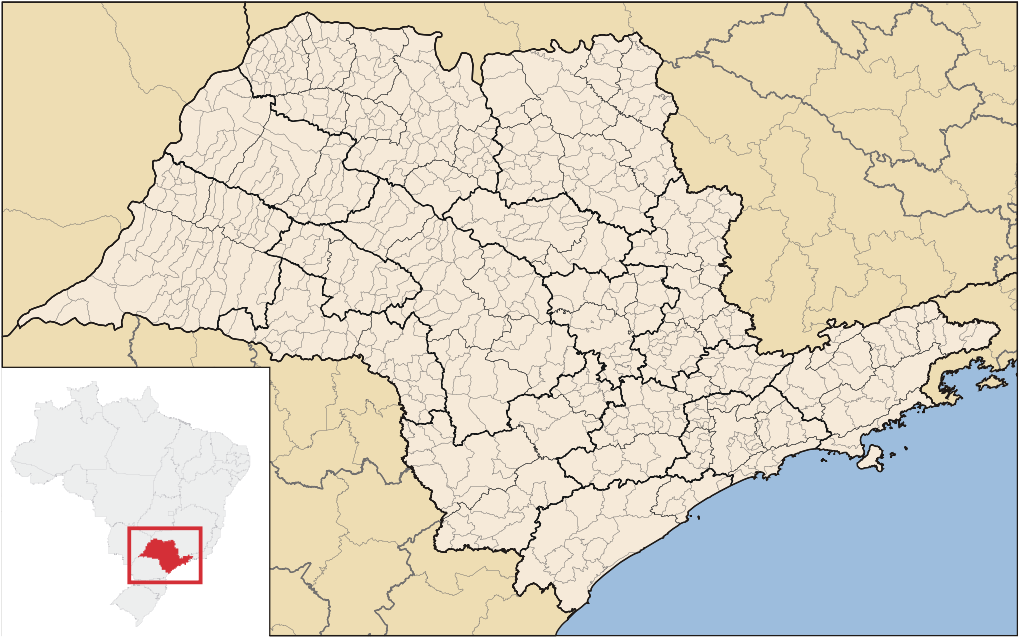
\includegraphics[width=\textwidth]{img/saopaulo_microregions.png}
	\caption{São Paulo state - cities, microregions and macroregions}
	\label{img_microregions}
\end{figure}

The open dataset PAM 2022 \cite{IBGEPAMProducao2022} provides a detailed assessment of Brazil's agricultural production.
The dataset contains information on planted area, harvested area and yearly production for all crops of commercial
interest at all cities in the country. Based on the total production, five cultures were selected as the most
representative of the Brazilian scenario. Each culture generates different agricultural residues
 \cite{souzaTheoreticalTechnicalAssessment2021} and has a specific urea consumption per unit of crop produced 
 \cite{IFASTATFertilizerUse2024}, with the results presented in \autoref{tab_biomasssupply}. 

\begin{table}
	\centering
	\caption{Biomass supply and urea demand for selected crops}
	\label{tab_biomasssupply}
	\begin{tabular}{|c | c | c | c | c|}
		\hline
		Crop & Biomass & Biomass supply \cite{souzaTheoreticalTechnicalAssessment2021} & Nitrogen Demand \cite{IFASTATFertilizerUse2024} \\
		 & & kg / kg crop & kg N / ha \\
		 \hline
		Sugarcane & Bagasse & 0.2200 & 76 \\ 
		 & Straw & 0.1848 &  \\
		Soybean & Straw & 0.6900 & 16 \\
		Corn & Stover & 0.6720 & 68 \\
		Rice & Husks & 0.6200 & 83 \\
		Coffee & Husks & 0.2950 & 161 \\
		\hline
	\end{tabular}
\end{table}

The provided biomass supply factors already take into account availability factors (actual residue available for energy
usage), save for the sugarcane bagasse, which is normally used to supply the necessary thermal energy (steam)
to a sugarcane mill. Therefore, for this study we considered only 24.2\% of the total bagasse to be available for
usage, corresponding to the surplus bagasse of a sugarcane plant processing sugarcane with 12\% fiber and a specific 
steam consumption of 400 kg steam / ton cane. 

In this way, the total biomass available per city can be evaluated by the total crop production, while the total urea
demand can be assessed by the planted area for each crop. The full, processed dataset is available at the supplementary
material.

\subsection{Process Model}

The full process topology is presented in \autoref{img_processtopology}. The process can be divided into the main subunits:
\begin{figure}
	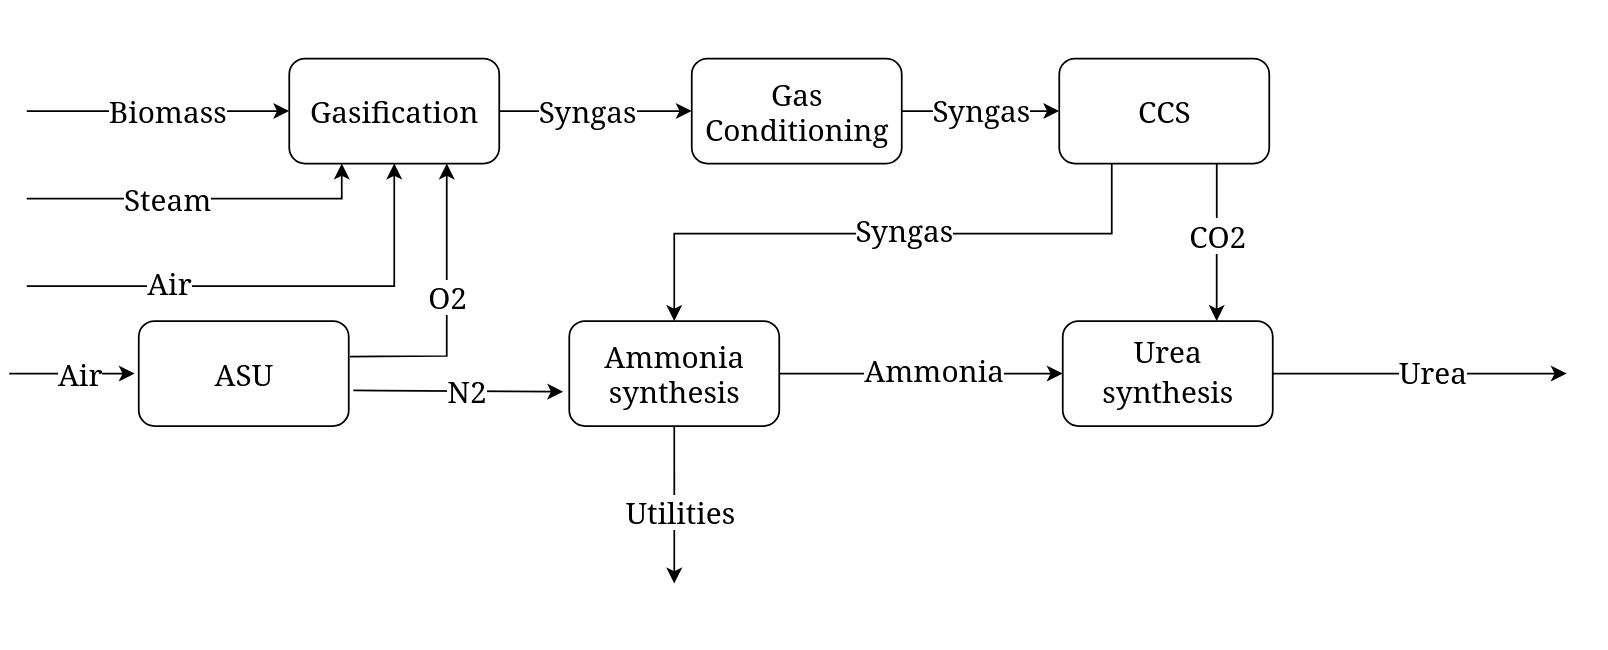
\includegraphics[width=\textwidth]{img/process_topology.png}
	\caption{Biomass gasification process flow diagram}
	\label{img_processtopology}
\end{figure}

\begin{itemize}
	\item Gasification
	\item Gas conditioning
	\item Carbon capture
	\item Ammonia Synthesis
	\item Urea Synthesis
	\item Air separation unit (ASU)
	\item Utilities 
\end{itemize}

\subsubsection{Biomass Gasification}

A process flow diagram of the gasification process is presented in \autoref{img_aspengasification}. Biomass was modeled
in Aspen Plus as a non-conventional component. \autoref{tab_biomass} presents the composition and heating value
of the main biomasses studied. 

\begin{figure}
	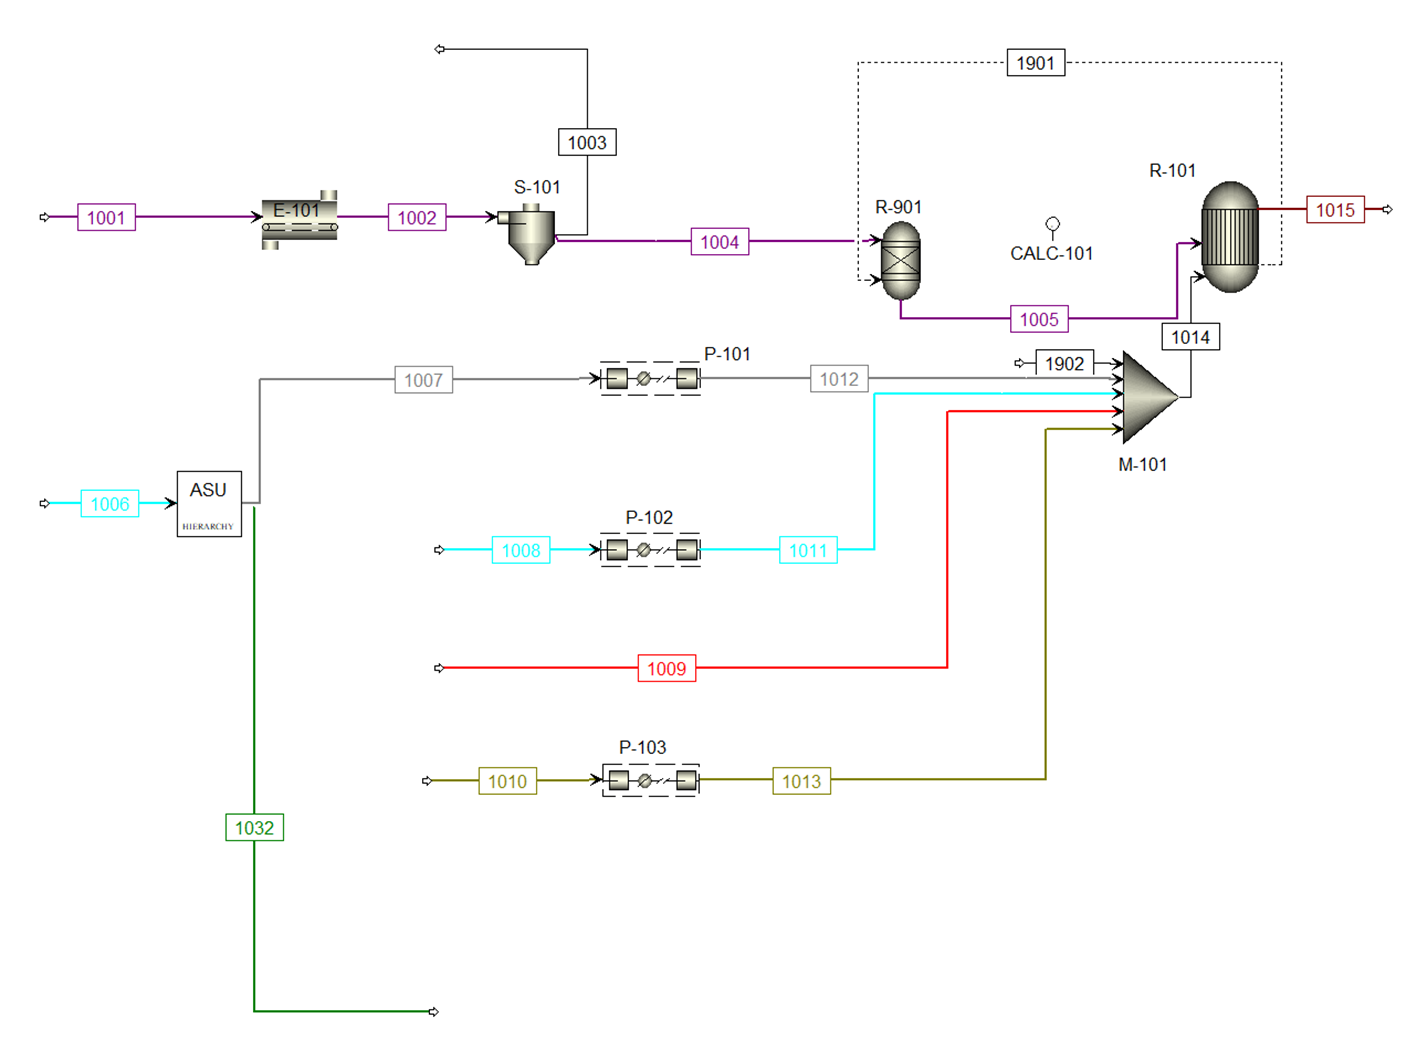
\includegraphics[width=\textwidth]{img/aspen_gasification.png}
	\caption{Biomass gasification process flow diagram}
	\label{img_aspengasification}
\end{figure}

\begin{sidewaystable}
	\caption{Biomass data}
	\label{tab_biomass}
	\begin{tabular}{||c | c | C{2.0cm} | C{2.0cm} | C{2.0cm} | C{2.0cm} | C{2.0cm} | C{2.0cm} ||}
		\hline
		 & & \multicolumn{6}{c||}{Biomass} \\
		\hline
		Name & Unit & Sugarcane bagasse \cite{jorapurSugarcaneLeafbagasseGasifiers1997} & Sugarcane straw \cite{jorapurSugarcaneLeafbagasseGasifiers1997} & Soybean straw \cite{tahirCatalyticFastPyrolysis2021} & Corn stover \cite{evansDevelopmentBiomassGasification1988} & Rice husk \cite{gaurAtlasThermalData1995} & Coffee husk \cite{anggonoCharacteristicsBiomassBriquettes2023} \\
		\hline
		Moisture & kg/kg \footnotemark[1] & 0.4000 & 0.2000 & 0.2000 & 0.2000 & 0.2000 & 0.2000 \\
		Ash & kg/kg \footnotemark[1]& 0.0420 & 0.0770 & 0.0530 & 0.0735 & 0.1580 & 0.0587 \\
		\hline
		C & kg/kg daf \footnotemark[2] & 0.4703 & 0.4312 & 0.5432 & 0.5025 & 0.4628 & 0.5221 \\
		H & kg/kg daf \footnotemark[2] & 0.0561 & 0.0596 & 0.0544 & 0.0628 & 0.0607 & 0.0569 \\
		O & kg/kg daf \footnotemark[2] & 0.4735 & 0.5071 & 0.3761 & 0.4287 & 0.4506 & 0.4066 \\
		N & kg/kg daf \footnotemark[2] & 0.0000 & 0.0021 & 0.0262 & 0.0060 & 0.0258 & 0.0143 \\
		\hline
		HHV & kJ/kg daf \footnotemark[2] & 18557 & 17430 & 18230 & 20500 & 18610 & 18795 \\
		\hline
	\end{tabular}

	\footnotetext[1]{As received}
	\footnotetext[2]{Dry and ash free}
\end{sidewaystable}
Biomass (1001) is received and dried to 15\% moisture in dryer E-101 by using low-pressure steam from the utilities
plant. 
Ash is separated at the solids separator and the biomass is converted from non-conventional into conventional 
components ($C$, $H_2$, $O_2$, $N_2$, $H_2O$) in a yield reactor (RYield) by using a calculator block. 
The decomposed biomass is mixed with the gasifying agents (pure oxygen, air, high-pressure steam and $CO_2$,
represented by streams 1007, 1008, 1009 and 1010, respectively) and gasified in the Gibbs reactor R-101.
Pure oxygen is supplied by the air separation unit, while $CO_2$ is supplied by the carbon capture system.

The gasification occurs on an entrained-flow gasifier, modeled using a non-stoichiometric equilibrium approach, 
due to its flexibility for comparing biomasses with different compositions 
\cite{gambarottaNonstoichiometricEquilibriumModel2018}. A global gasification reaction can be described as:

\begin{multline}
	CH_aO_bN_c + wH_2O_{(l)} + sH_2O_{(g)} + e(O_2+\rho N_2) + dCO_2 \rightleftharpoons n_{CH_4}CH_4 \\ 
	+ n_{CO_2}CO_2 + n_{CO}CO + n_{H_2}H_2 n_{H_2O}H_2O + n_{O_2}O_2 + n_{N_2}N_2
\end{multline}

With $a$, $b$ and $c$ being derived from the biomass composition; $w$, $s$, $e$, $\rho$ and $d$ representing the
gasifying agent mixture, and $n_i$ being the number of moles of component $i$ in the syngas. At equilibrium, the Gibbs
energy of the mixture ($G$) must be at minimum.

\begin{equation}
	G = \sum_{i=1}^{M}{n_iG_i^0} + \sum_{i=1}^{M}{n_iRT ln \left( \frac{n_i}{n_{tot}} \right) }
\end{equation}

The number of moles of each component, $n_i$, are constrained by the mole balance of each atom C, H, O and N on the
biomass. Tar formation is not considered in this model. The minimization of Gibbs energy is obtained on the Gibbs 
reactor block (RGibbs). Syngas properties were calculated using the Peng-Robinson equation of state, 
with Boston-Mathias modifications. The gasification conditions are initially set to 30 bar of pressure and a 
temperature of 1200°C.  The temperature is controlled by the oxygen injection on the gasifier. All other gasifying 
agents are parameters of the model.

\subsubsection{Air separation unit}

A process flow diagram of the air separation unit is presented in \autoref{img_aspenasu}. 
Air is compressed in a multistage compressor (P-501) to an intermediate pressure of 6 bar and split into 2 streams. 
One stream (5003) is further compressed in compressor P-502 to a higher pressure of 7.5 bar and liquefied in a 
multi-stream heat exchanger using the products from the distillation section. 
The lower pressure air stream (5010) is cooled in the same heat exchanger and used as the vapor feed for the 
high-pressure column operating at 6 bar.
A rich nitrogen stream is removed as the distillate fraction from the HP column (5014), while the bottom fraction is 
a rich oxygen mixture (5015). 
Both streams are further cooled in a second multi-stream heat exchanger and sent to the low-pressure column operating
at 1.8 bar for further separation. The rich nitrogen fraction is fed at the top of the column while the rich oxygen 
fraction is fed at an intermediate stage. The columns are thermally coupled in the sense that the reboiler duty of the
low-pressure section is the condenser duty from the high-pressure section, and the liquefied air expansion is the 
thermal drive for the separation.

The system is designed to produce $N_2$ with 99.5\% mole fraction and $O_2$ with 99\% mole fraction. These purities
are achieved by manipulating the high-pressure/low-pressure split at S-501, and the high-pressure column 
reflux ratio in design specifications. The $O_2$ is sent directly to the gasification system, while the $N_2$ is 
partially sent to the ammonia synthesis unit while the excess is compressed and sold as a separate product.

\begin{figure}
	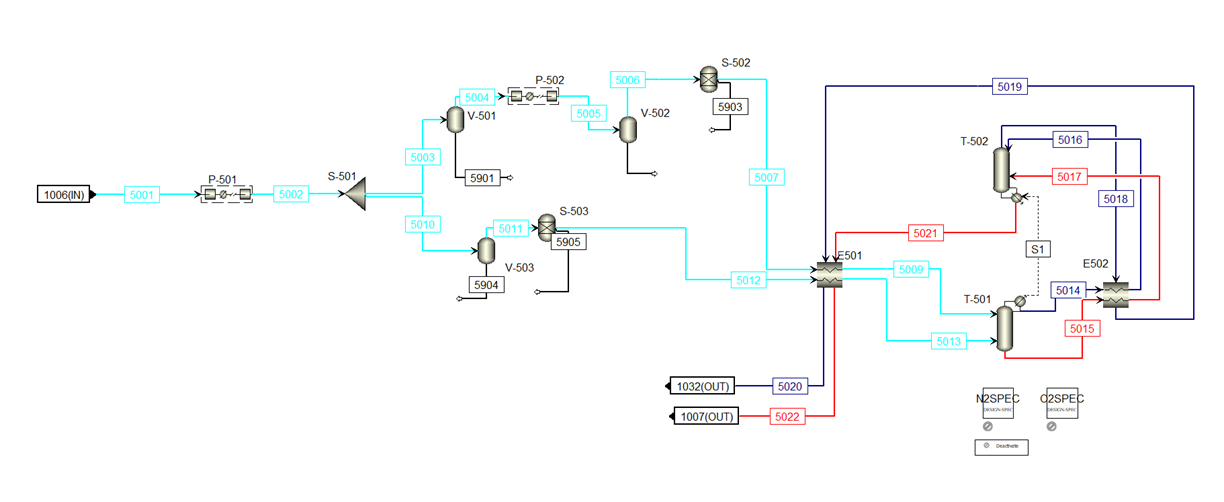
\includegraphics[width=\textwidth]{img/aspen_asu.png}
	\caption{Air separation unit (ASU) process flow diagram}
	\label{img_aspenasu}
\end{figure}

\subsubsection{Gas Conditioning}

A process flow diagram of the gas conditioning unit is presented in \autoref{img_aspenconditioning}

\begin{figure}
	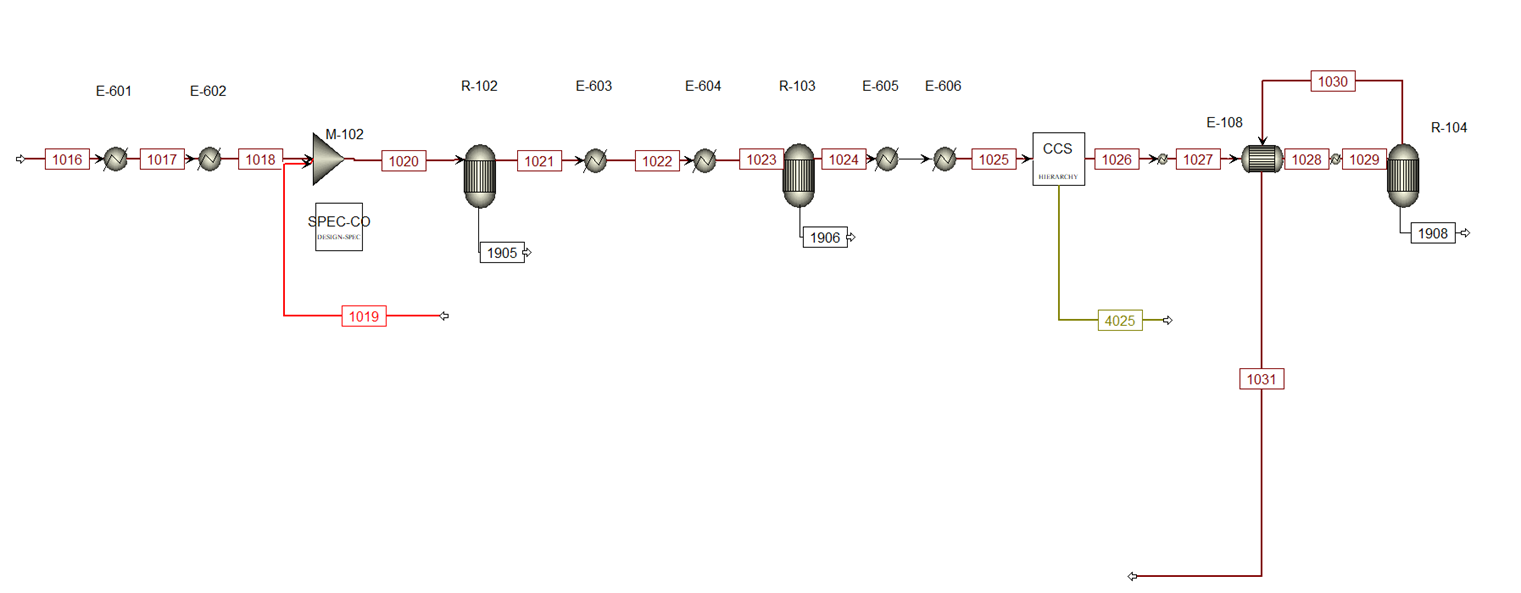
\includegraphics[width=\textwidth]{img/aspen_conditioning.png}
	\caption{Gas conditioning unit process flow diagram}
	\label{img_aspenconditioning}
\end{figure}

The syngas from the gasification plant is rich in both $H_2$ and $CO$. Given that $CO$ is undesired in the 
ammonia synthesis, a gas conditioning unit is designed to maximize the $H_2$ concentration on the syngas by leveraging 
the water-gas shift reaction. This reaction can be described as:

\begin{equation}
	CO + H_2O \rightleftharpoons CO_2 + H_2 \quad \Delta H_{ref}^0 = -41 kJ/mol
\end{equation}

The water-gas shift reaction is exothermic and driven by equilibrium, which means that low temperatures favor the
product formation. At the same time, the reaction kinetics is favorable in high temperature, which means that there's 
a trade-off between $CO$ conversion and reactor size \cite{florez-orregoProcessSynthesisOptimization2018}. Therefore, 
the chosen design uses two shift reactors operating with inlet conditions of 310°C and 210°C, and intermediate cooling.

The hot syngas from the gasification section (1016) is cooled to 310°C in two utility heat exchangers
(E-602 and E-603), generating high pressure superheated steam. The syngas is then mixed with high pressure steam 
(1019) produced in the utility unit and sent to the high temperature shift reactor (R-102). The partially shifted 
syngas is cooled to 210°C into 2 intermediate heat exchangers (E-603 and E-604), also connected to the utilities 
plant, and sent to the low temperature shift reactor (R-103) for further $H_2$ generation. The syngas is cooled yet 
again at 2 utility heat exchangers (E-605 and E-606), to maximize the heat recovery of the process.

The $CO_2$ on the syngas (4025) is captured at the carbon capture and storage (CCS) unit, described in the next 
section. After the $CO_2$ capturing, the final step in the gas conditioning is to remove any remaining $CO$ and $CO_2$
in the syngas, considering that both molecules are poisons to the ammonia catalysts. This is done in a methanation 
reactor (R-104). The methanation reaction is also equilibrium-driven and can be described as:
\begin{alignat}{2}
	&CO + 3H_2 \rightleftharpoons CH_4 + 3H_2O \quad & &\Delta H_{ref}^0 = -206 kJ/mol \\
	&CO_2 + 4H_2 \rightleftharpoons CH_4 + 4H_2O \quad & &\Delta H_{ref}^0 = -164 kJ/mol
\end{alignat}


These reactions consume $H_2$ and generate $CH_4$, which is an inert on the ammonia loop. Therefore, they are undesired 
for the process.

The steam injection at the start of the process is a design specification of the model and is set to control the mole
fraction of $CO$ at the CCS inlet (1025) to below 0.5\%. Syngas properties for this unit were calculated using 
the Peng-Robinson equation of state, with Boston-Mathias modifications.

\subsubsection{Carbon capture}

A process flow diagram of the carbon capture and storage unit is presented in \autoref{img_aspenccs}.
A physical absorption system using DEPG (dimethyl ethers of polyethylene glycol) was chosen for this step, widely
used for $CO_2$ capture in gasification for syngas production. The proposed system is based on the optimized design
of \textcite{martelliMultiobjectiveOptimizationSelexol2015} and modified for the biomass gasification specific needs. 

\begin{figure}
	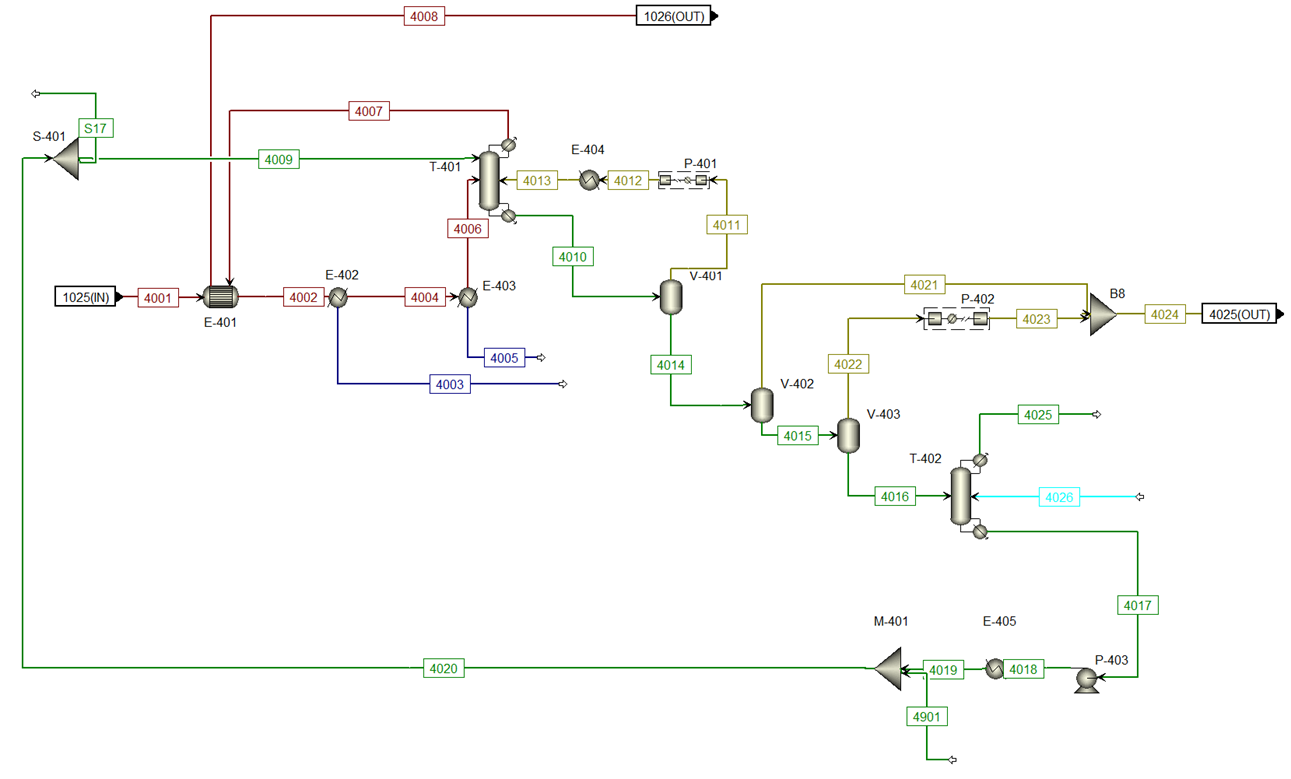
\includegraphics[width=\textwidth]{img/aspen_ccs.png}
	\caption{Carbon capture unit process flow diagram}
	\label{img_aspenccs}
\end{figure}

The syngas (4001) at 30 bar is cooled to 4°C in 3 stages by using purified syngas (E-401), cooling water (E-402) and
chiller water (E-403) and sent to the absorber column (T-401) where it gets in contact with the $CO_2$-lean 
solvent (4009). The $CO_2$ on the rich solvent (4010) is removed in a series of flash drums (V-401 to V-403). 
The gas from the first flash drum (4011) is rich in $H_2$ and is therefore recirculated back to the absorber column,
while the gas phase from the other drums is compressed to be used in the urea synthesis, with the remaining fraction sold as a byproduct. After all expansions, the solvent is finally stripped with air \cite{mokhatabNaturalGasSweetening2012} 
in column T-402 for deep removal of $CO_2$ still present on the solvent; this step ensures the $CO_2$ content of the 
purified syngas stays at minimal levels, and therefore minimizes $H_2$ consumption on the methanation reactor. 
The stripped solvent (4017) is cooled to -1°C and recirculated back to the absorber column.

The physical properties of the DEPG-$CO_2$ equilibrium were estimated by using the PC-SAFT equation of state
\cite{dymentAcidGasCleaning2015}.

\subsubsection{Ammonia synthesis}

Ammonia is synthesized on the traditional Haber-Bosch process, developed in 1909 and still used on an industrial scale.
The ammonia synthesis reaction is:

\begin{equation}
	N_2 + 3H_2 \rightleftharpoons 2NH_3 \quad \Delta H_{ref}^0 = -92.4 kJ/mol
\end{equation}

As this is an exothermic equilibrium-driven reaction, high temperatures are unfavorable to the formation of products.
In the customary process temperatures, conversion from syngas into ammonia is only 25-35\% per pass in the catalyst
\cite{applAmmoniaPrinciplesIndustrial1999}. A pressure increase also dislocates the equilibrium to the product as it 
has less gas moles \cite{sandlerChemicalBiochemicalEngineering2017} at the same time where it raises the power 
consumption for the syngas compression and recirculation. There is a trade-off between process yield, reactor size and 
power consumption of the unit that must be taken into account.

The ammonia synthesis kinetics implemented in this model is that proposed by 
\textcite{singhSimulationAmmoniaSynthesis1979}, which modifies the traditional Temkin-Pyzhev equation 
\cite{temkinKineticsAmmoniaSynthesis1940} by incorporating the gas non-ideality by replacing the partial pressure 
with fugacity. The parameters for this kinetic formulation were regressed from real performance data for two 
commercial catalysts (Montecatini-Edison and Haldor Topsøe). The reaction rate is represented as:

\begin{align}
	&r = k_0 \left[ k_a^2f_{N_2} \left(  \frac{f^3_{H_2}}{f^2_{NH_3}} \right)^{0.55} - \left( \frac{f^2_{NH_3}}{f^3_{H_2}} \right)^{0.45} \right] \\
	&k_0 = \exp \left(2.303 \cdot 14.7102 - \frac{39057}{RT}\right)
\end{align}

With $k_a$ being the equilibrium constant of the reaction, obtained experimentally by 
\textcite{gillespieThermodynamicTreatmentChemical1930} and represented as:

\begin{multline}
	\log_{10}k_a = -2.691122\log_{10}T - 5.519265\cdot10^{-5}T \\
	 + 1.848863\cdot10^{-7}T^2 + \frac{2001.6}{T} + 2.6899
\end{multline}

\textcite{florez-orregoProcessSynthesisOptimization2018} studied a variety of configurations for the ammonia synthesis
with an energy and exergy efficiency analysis and obtained an optimal configuration of operational parameters and 
energy integrations, chosen as the starting point for this study. A process flow diagram of the ammonia synthesis 
unit is presented in \autoref{img_aspennh3}.

\begin{figure}
	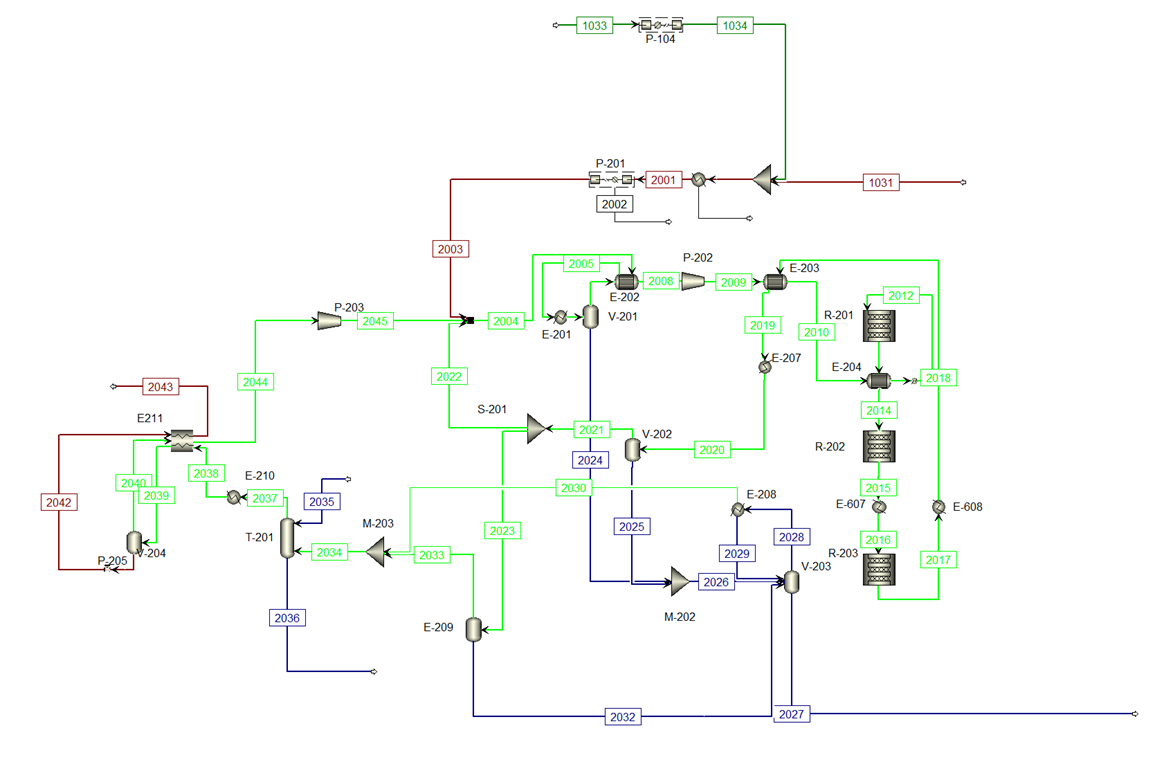
\includegraphics[width=\textwidth]{img/aspen_nh3.png}
	\caption{Ammonia synthesis process flow diagram}
	\label{img_aspennh3}
\end{figure}

Syngas from the gasification and gas conditioning (1031) is mixed with nitrogen from the air separation unit (1033), 
maintaining a molar $H_2/N_2$ ratio of 2.9:1. The syngas is compressed to the process pressure of 200 bar and sent to 
the loop, where it is mixed with the recycle gases (2022) and the rich $H_2$ gas from the purge gas treatment. 
The gas mixture is chilled to -20°C in heat exchangers (E-202 and E-201). The liquid is separated in flash drum 
(V-201), while the gas phase is sent to the circulation compressor (P-202), designed to withstand the pressure loss 
of the system. 

The compressed gases (2009) are sent to the reactor; they are pre-heated to 310°C utilizing the outlet gas from the 
reactor (2018) and first reactor beds (2013), and sent to the first bed. The reactor possesses three catalytic beds, 
R-201/202/203, operating with inlet temperatures of 310°C, 420°C and 380°C. This inlet temperature is maintained by 
indirect intermediate cooling between each bed, to leverage the favorable equilibrium conditions at lower temperatures.
Between the first and second bed, the gas is cooled by the reactor feed, while the heat exchangers E-607 and E-608 cool
the gases by generating steam in the utility plant. 

After all heat recoveries, the reactor outlet stream (2019) is cooled to 30°C with cooling water on E-207. Most of the 
liquid $NH_3$ is recovered on this first cooling stage. The gas phase of separation drum V-202 (2021) is recycled back
into the process, except for a purge fraction (2023) of 3\% of the total loop flow. This purge is designed to keep the
total inert molar fraction in the ammonia loop close to 10\%, as the inerts reduce the reactants conversion and
increase the circulation rate \cite{florez-orregoProcessSynthesisOptimization2018}. 
The liquid $NH_3$ from both condensers (2024, 2025) is expanded to 80 bar to recover a rich $H_2$ stream (2030) and
the final $NH_3$ product (2027) is sent to the urea synthesis unit.

The loop purge gas (2023) contains a about 60\% mol of $H_2$, which is recovered on the cryogenic purge gas treatment 
section. The gas is chilled to -20°C to recover any liquid ammonia not condensed in the main loop and mixed with the
rich $H_2$ gases from the $NH_3$ flashing (2030). The remaining $NH_3$ is removed in the absorber column T-201, 
using water to produce an aqua-ammonia stream (2036). The outlet gases from the absorber (2037) are again cooled to
-20°C  in heat exchanger E-210, and refrigerated to -192°C in the cold box E-211, where the majority of the non-$H_2$
components such as $CH_4$ and $N_2$ condense. The liquid fraction of the outlet mixture is separated in the flash drum V-204 and expanded to atmospheric pressure to drive the inlet gas cooling. The recovered rich $H_2$ stream (2044) is re-compressed
and sent back to the ammonia loop, while the $CH_4$-rich stream (2043) is sent to the utilities plant.

The gas properties for this unit were calculated using the Peng-Robinson equation of state with Boston-Mathias
modifications.

\subsubsection{Urea synthesis}
The urea synthesis consists of the formation of ammonium carbamate, and its dehydration into urea, and can be
represented by the following reactions:

\begin{alignat}{2}
	&2NH_3 + CO_2 \rightleftharpoons NH_4NH_2CO_2 \quad & &\Delta H_{ref}^0 = -117 kJ/mol  \\
	&NH_4NH_2CO_2 \rightleftharpoons (NH_2)_2CO + H_2O \quad & &\Delta H_{ref}^0 = +15.5 kJ/mol 
\end{alignat}

Both reactions occur exclusively in the liquid phase. The carbamate formation is strongly exothermic and fast, while 
the urea formation is slow and slightly endothermic, and is therefore the determining step of the process.

For this study, $CO_2$-stripping process based on the commercial Stamicarbon® technology was chosen 
\cite{meessenUreaSynthesis2014}. A process flow diagram of the urea unit is presented in \autoref{img_aspenurea}.

\begin{figure}
	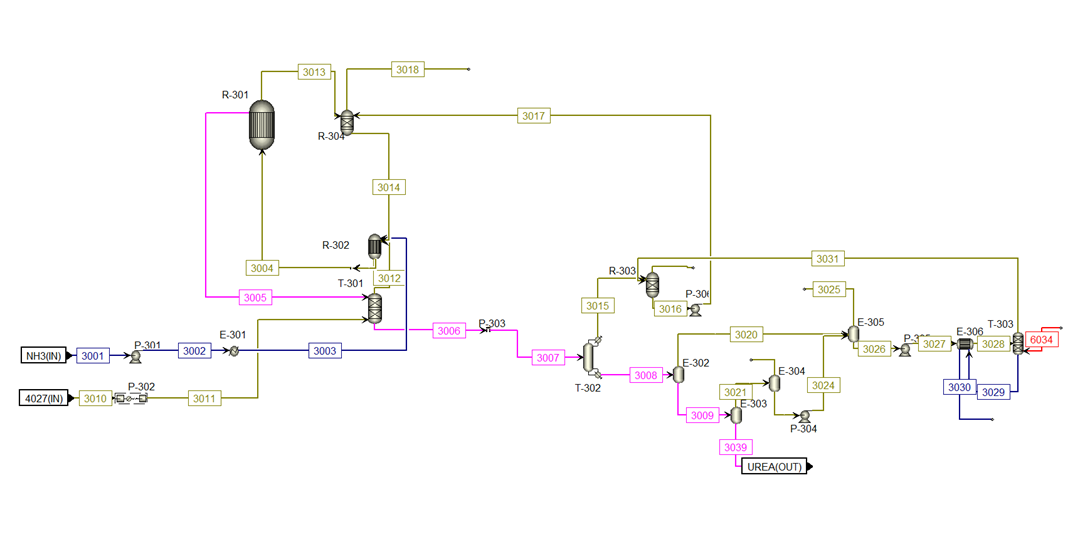
\includegraphics[width=\textwidth]{img/aspen_urea.png}
	\caption{Urea synthesis process flow diagram}
	\label{img_aspenurea}
\end{figure}

$NH_3$ (3001) is received from the ammonia synthesis unit and $CO_2$ (3010) is received from the CCS unit. They are 
both compressed to the process pressure of 140 bar. The $CO_2$ is used as the stripping agent on the carbamate 
stripper T-301, which is essentially a high-pressure heat exchanger. The stripper decomposes the unreacted carbamate 
from the urea reactor back into $NH_3$ and $CO_2$, using medium pressure steam to drive the decomposition. The vapor 
mixture from the stripper (3012) is partially re-condensed into carbamate on the high-pressure condenser, R-302, 
operating at 167°C. As with the stripper, the condenser is also a high-pressure heat exchanger. Since carbamate 
formation is highly exothermic, the condenser is cooled by boiler feedwater, directly generating low-pressure steam.
The extent of condensation is controlled by changing the water level inside the condenser, as to guarantee that a 
small amount of $NH_3$ and $CO_2$ condenses on the urea reactor to control the temperature at the reactor and 
drive the endothermic synthesis.

The reactor (R-301) is modeled as a two-phase plug-flow reactor. The liquid phase (3005) returns to the stripper, 
while the vapor phase (3013) is absorbed in the high-pressure scrubber R-304, using recovered carbamate solution from 
the low-pressure condenser.

The urea solution from the stripper (3006) is concentrated in a reactive distillation column (T-302) operating at 
4.5 bar and 135°C, where the remaining carbamate is decomposed, together with any volatile components. The gas phase 
from the column (3015) is condensed back into carbamate in the low-pressure condenser, R-303, and circulated back to 
the high-pressure scrubber. The liquid from the distillation column (3008) is urea at 75 wt\%, with the remaining 
components being water and a small amount of liquid ammonia. The urea is concentrated to 99 wt\% in a double effect 
evaporator (E-302/303) operating at 80 mbar and 140°C, driven by low-pressure steam. The condensate from the 
evaporators (3026) is contaminated with $NH_3$, which is removed in a stripper (T-303), with the $NH_3$-rich vapors 
(3031) being sent back to the low-pressure condenser. The final urea stream (3039) is sent to a granulation or 
prilling unit.

The fluid properties for this unit were calculated using the SR-POLAR equation of state 
\cite{aspentechASPEN88Technical2011}.

\subsubsection{Utilities}

A process flow diagram of the utilities plant is presented in \autoref{img_aspenutilities} and
\autoref{img_aspenrefrigeration}.

\begin{figure}
	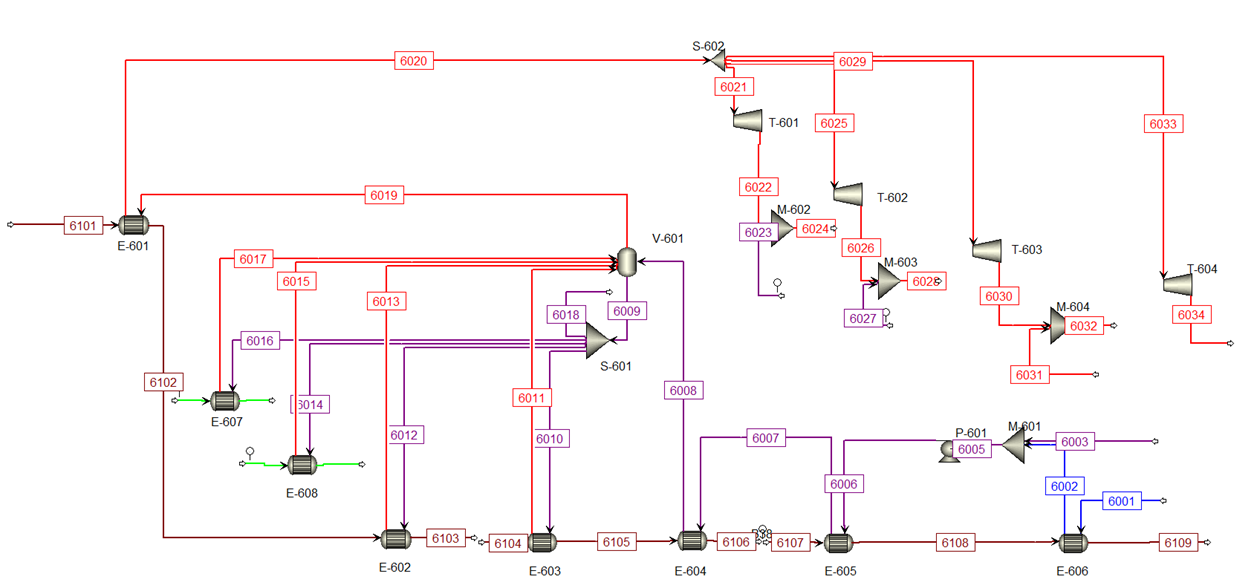
\includegraphics[width=\textwidth]{img/aspen_utilities.png}
	\caption{Utilities plant}
	\label{img_aspenutilities}
\end{figure}
\begin{figure}
	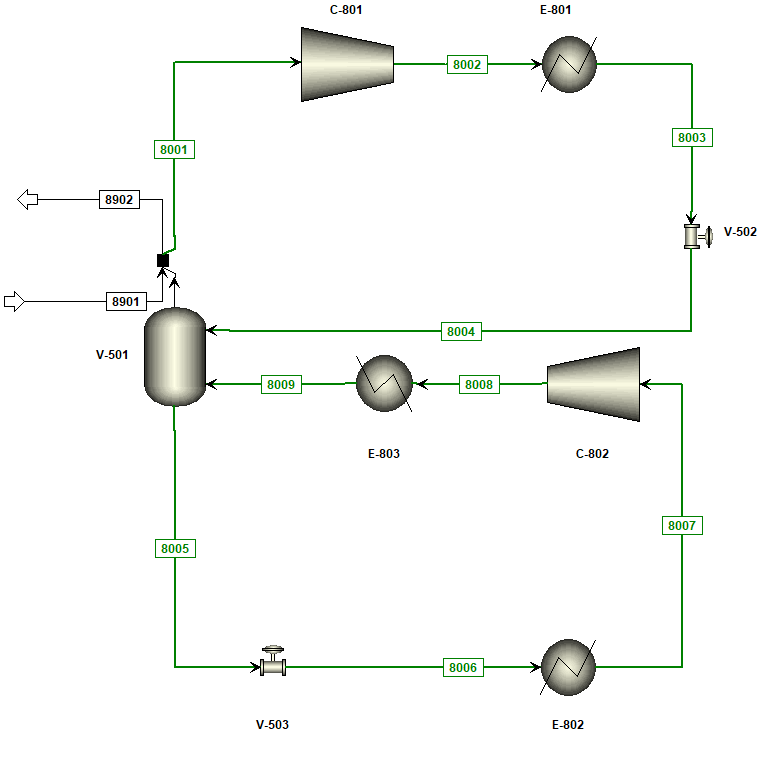
\includegraphics[width=\textwidth]{img/aspen_chiller.png}
	\caption{Refrigeration plant}
	\label{img_aspenrefrigeration}
\end{figure}


The unit is designed to generate steam at 90 bar and 510°C. Makeup water is preheated in economizer E-606, mixed with
process condensate in a deaerator, and further heated in economizers R-605 and E-604. Saturated steam is generated in 
evaporators E-603/E-602 using syngas, and E-606/E-607 using ammonia loop gases. The steam is superheated to 510°C 
in heat exchanger E-601 and sent to a steam turbine with 3 extraction stages. 

High pressure steam (6024) is extracted at 30 bar to be used in the gas conditioning unit. Medium pressure steam at 
15 bar is extracted to be used in the urea stripper T-301. Low-pressure steam at 4.5 bar is extracted (6030) and mixed 
with steam generated at the urea high-pressure condenser (6031), to be used in the rest of process heating 
applications., primarily in the biomass drying and urea concentration. The remaining steam is condensed at 0.1 bar.  

A two-stage refrigeration system with intercooling \cite{stoeckerIndustrialRefrigerationHandbook2004} was modeled 
separately from the utilities plant. Refrigerant R-717 (ammonia) is compressed to 15 bar at compressor C-801, 
condensed at condenser E-801 using cooling water and expanded to an intermediate pressure of 3.87 bar at valve V-502. 
The vapor-liquid mixture is collected in vessel V-501. The liquid collected at this vessel is expanded to a pressure
of 1.1 bar and the resultant vapor-liquid mixture is completely evaporated at evaporator E-802, providing the chiller
heat load for the plant. The vapors are recompressed to 3.87 bar at the low pressure compressor, intercooled with 
cooling water and recycled back into the intermediate vessel. The vapors from this vessel are sent back to the 
high pressure compressor.

The resulting refrigeration system presents a COP (coefficient of performance) of 2.75. To decouple the chiller model
from the main process model, this COP is used to obtain power consumption for all cases based on the required chilling
load.


\subsection{Supply-chain model}

A mixed-integer linear programming (MILP) optimization modeling framework was built using the Pyomo open-source
software suite, with the objective of obtaining the ideal location and capacity of a renewable urea plant,
based on the process model performance, local biomass supply and urea demand. The model can be divided into 4 layers,
represented in \autoref{img_layers}.

\begin{figure}
	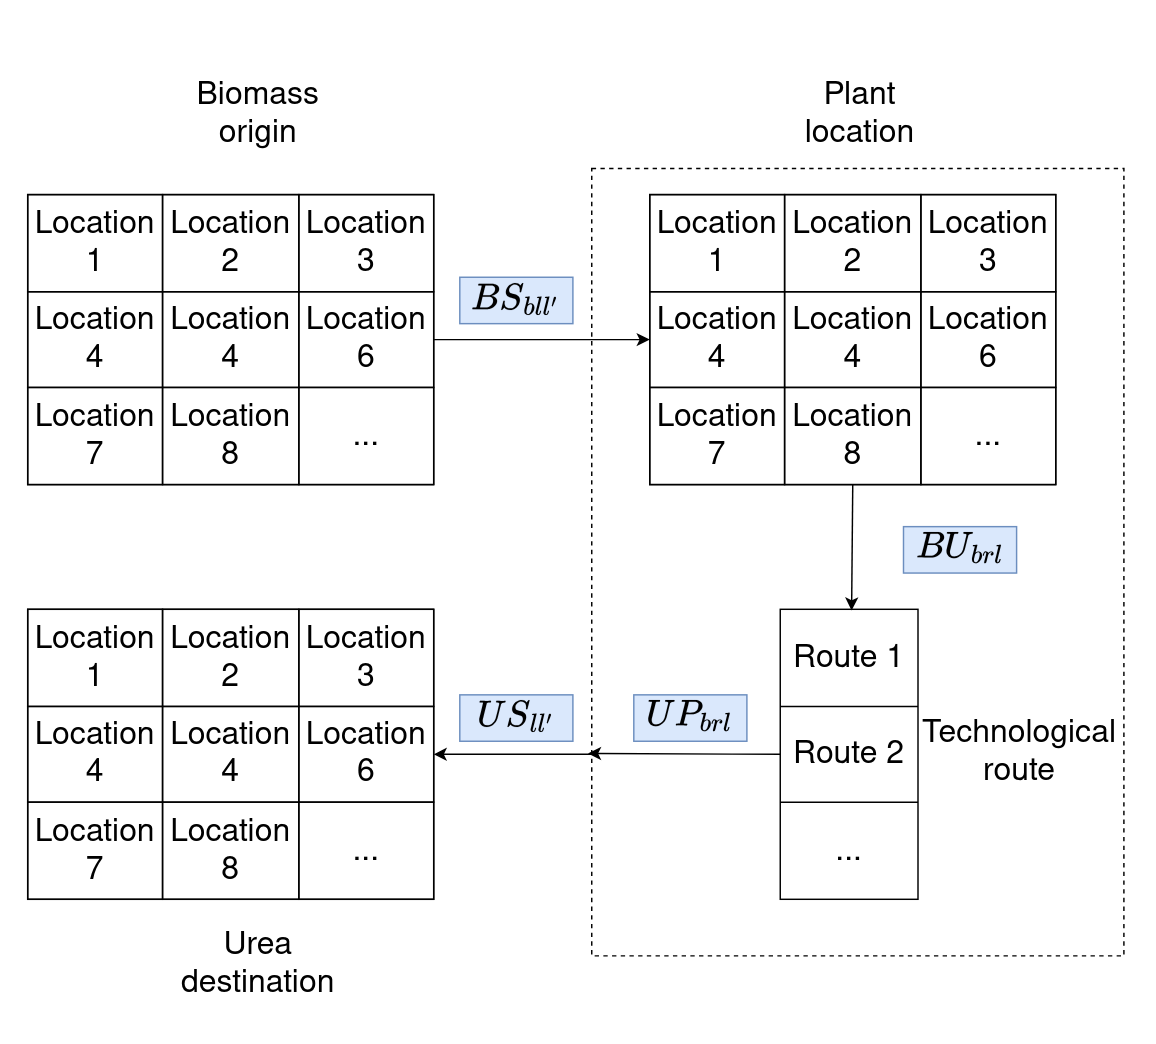
\includegraphics[width=\textwidth]{img/layers_of_decision.png}
	\caption{Layers of decision for the supply-chain model}
	\label{img_layers}
\end{figure}

The model consists of 3 main sets:

\begin{itemize}
	\item L: set of possible locations ($l$)
	\item B: set of possible biomasses ($b$)
	\item R: set of technological routes for urea production (e.g.: pure oxygen gasification vs. air mixed gasification)
\end{itemize}

Based on these sets, the decision variables of the model are:

\begin{itemize}
	\item $BS_{bll'}$: Biomass $b$ sold from location $l$ to location $l'$ (tons/year)
	\item $BU_{brl}$: Biomass $b$ used through route $r$ at location $l$ (tons/year)
	\item $UP_{rl}$: urea produced via route $r$ at location $l$ (tons/year)
	\item $US_{ll'}$: urea sold from location $l$ to location $l'$ (tons/year)
	\item $PU_{rl}$: power used through route $r$ at location $l$ (MWh/year)
	\item $W_l$: binary variable corresponding to the installation of the plant at location $l$
	\item $C$: capacity of the plant (tons urea / h)
	\item $CAPEX$: capital costs of the plant (MMUSD)
\end{itemize}

The user-supplied parameters of the model are:
\begin{itemize}
	\item $S_{bl}$: supply of biomass $b$ at location $l$
	\item $DU_l$: urea demand at location $l$
	\item $CV_{br}$: conversion of biomass $b$ to urea using route $r$ (in t urea / t biomass)
	\item $PR_{br}$: utility (power) requirements of producing urea with biomass $b$ at route $r$ (in MWh / t biomass)
	\item $CB_{bl}$: cost of biomass $b$ at location $l$
	\item $PP_l$: power price at location $l$
	\item $PU_l$: urea price at location $l$
	\item $D_{ll'}$: distance from location $l$ to location $ll'$
	
\end{itemize}

The model assumes that a single plant will be installed in a location. Biomass can be originated from any of the 
possible locations, and sold to the plant. The plant can process the combination of biomasses into any technological
route available, producing urea, which can then be sold back to any of the possible locations. 

The main constraints of the model are described as following. A plant can only be installed at a single location:

\begin{equation}
	\sum_{l \in L} W_l = 1
\end{equation}

If a plant is not installed at a location, then the urea produced at that location must be zero:

\begin{equation}
	\sum_{r \in R} UP_{rl} <= M \cdot 8585 \cdot W_l \quad \forall \ l \in L
\end{equation}

Total urea produced must be equal to the plant's capacity:

\begin{equation}
	\sum_{r \in R} \sum_{l \in L} UP_{rl} = C \cdot 8585
\end{equation}

The total urea produced at one site must be equal to the total urea sold from that site to all locations:

\begin{equation}
	\sum_{r \in R} UP_{rl} = \sum_{l' \in L} US_{ll'} \quad \forall \ l \in L
\end{equation}

Biomass consumed is proportional to urea produced and the corresponding conversion factors:

\begin{equation}
	UP_{rl} = \sum_{b \in B} BU_{brl} \cdot CV_{br} \quad \forall \ (r \in R, \ l \in L)
\end{equation}

Power consumed is also proportional to urea produced:

\begin{equation}
	PU_{rl} = \sum_{b \in B} BU_{brl} \cdot PR_{br} \quad \forall \ (r \in R, \ l \in L)
\end{equation}

Biomass used must be equal to the total biomass sold to the plant's location:

\begin{equation}
	\sum_{r \in R} BU_{brl} = \sum_{l' \in L} BS_{bl'l} \quad \forall \ (b \in B, \ l \in L) 
\end{equation}

Total biomass sold from a location must be lower than the biomass supply:

\begin{equation}
	\sum_{l' \in L} BS_{bll'} <= S_{bl} \quad \forall \ (b \in B, \ l \in L)
\end{equation}

Total urea sold to a location must be lower than the urea demand:

\begin{equation}
	\sum_{l' \in L} US_{l'l} <= DU_l \quad \forall \ l \in L 
\end{equation}

CAPEX is calculated based on the capacity by piecewise linearization of the estimated CAPEX at reference capacities of
20, 35, 50 and 80 tons urea / h.

The objective function of the model is to maximize the NPV of the plant. The maximum capacity was initially constrained
to 80 t/h, corresponding roughly to 10\% of the national demand for 2022.


\subsection{Economical evaluation}
The capital costs for all subunits of the process were estimated by using the methodology proposed by
\textcite{turtonAnalysisSynthesisDesign2018}:

\begin{equation}
	C = C_{ref} \cdot \left( \cfrac{A}{A_{ref}} \right)^n \cdot \cfrac{CEPCI}{CEPCI_{ref}}
\end{equation}

With $C$ and $C_{ref}$ being the capital cost of the actual and reference unit, $A$ and $A_{ref}$ being the equipment
cost attribute (capacity) for the actual and reference unit, and $CEPCI$ being the Chemical Engineering Plant
Cost Index for the current and reference year. The reference costs include auxiliaries and erection. An additional
30\% of the total estimated capital cost is assumed for auxiliaries and other equipment not included in any scope,
while 25\% is separated for contingencies.

\autoref{tab_capex} summarizes the capital costs for all subunits of the plant, designed to produce 99 wt.\% of urea. 
A reference capacity of 35 t / h was chosen for this summary.

\begin{sidewaystable}
	\caption{Capital cost estimation}
	\label{tab_capex}
\begin{tabular}{|| C{2.3cm} | c | c | c | c | C{1.4cm} | C{1.2cm} | c | c | C{0.9cm} | C{1.4cm} | C{1.5cm} | C{0.9cm} ||}
		\hline
		CAPEX Estimation & \multicolumn{2}{c |}{Reference cost} & \multicolumn{2}{c |}{Reference capacity}
		& Reference date & CEPCI (ref.) & \multicolumn{2}{c |}{Current capacity} & Scale factor & Includes
		auxiliaries & Adjusted CAPEX (MMUSD) & Source \\
		\hline
		Ammonia unit & 18 & MMEUR & 175000 & t urea / year & 2017 & 567.5 & 300483 & t urea / year & 0.64 & Yes & 39.6
		& \cite{antonettiWastetoChemicalsCircularEconomy2017} \\
		Urea unit & 28 & MMEUR & 175000 & t urea / year & 2017 & 567.5 & 300483 & t urea / year & 0.64 & Yes & 61.6 &
		\cite{antonettiWastetoChemicalsCircularEconomy2017} \\
		Methanator & 3.3 & MMEUR & 522900 & t $NH_3$ / year & 2021 & 720.2 & 166654 & t $NH_3$ / year & 0.85 & Yes & 1.5 &
		\cite{cloeteCosteffectiveCleanAmmonia2021} \\
		WGS Unit & 6.6 & MMEUR & 522900 & t $NH_3$ / year & 2021 & 720.2 & 166654 & t $NH_3$ / year & 0.85 & No & 5.5 &
		\cite{cloeteCosteffectiveCleanAmmonia2021} \\
		CCS & 12 & MMUSD & 3000 & t solvent / h & 2015 & 556.8 & 950 & t solvent / h & 0.6 & No & 15.6 &
		\cite{imEconomicAssessmentOptimization2015} \\
		ASU & 46.3 & MMUSD & 6.7 & kg $O_2$ / s & 2021 & 720.2 & 5.3 & kg $O_2$ / s & 0.8 & Yes & 42.8 &
		\cite{cloeteCosteffectiveCleanAmmonia2021} \\
		Gasification & 67.8 & MMUSD & 2222 & t bio / day & 2011 & 550.8 & 1038 & t bio / day & 0.6 & Yes & 62.6 &
		\cite{swansonTechnoeconomicAnalysisBiomasstoliquids2010} \\
		Power plant & 17.9 & MMEUR & 38.7 & MW & 2021 & 720.2 & 12 & MW & 0.8 & Yes & 8.6 &
		\cite{cloeteCosteffectiveCleanAmmonia2021} \\
		\hline
		Total & 237.9 & MMUSD & & & & & & & & & & \\
		Auxiliaries & 71.4 & MMUSD & & & & & & & & & & \\
		Contingencies & 59.5 & MMUSD & & & & & & & & & & \\
		\hline
		Total & 368.7 & MMUSD & & & & & & & & & & \\
		\hline
	\end{tabular}

\end{sidewaystable}

Operational, maintenance and insurance labor costs were considered as a fixed percentage of the total capital cost.

Net present value (NPV) is defined as:

\begin{equation}
	NPV = \sum_{t=1}^n \cfrac{F_t}{(1+r)^t}
\end{equation}

Urea levelized cost has been calculated as follows:

\begin{equation}
	LC = \cfrac{NPV_{costs}}{NPV_{output}} = \cfrac{\displaystyle\sum_{t=1}^n \cfrac{C_t + O_t}{(1+r)^t}}{\displaystyle\sum_{t=1}^n \cfrac{U_t}{(1+r)^t}}
\end{equation}

With $F_t$ being the net cash flow at year t, $C_t$ being the capital expenditures at year t, $O_t$ being the
operational and fuel expenses at year t, $U_t$ being the total urea produced, and $r$ being the discount rate,
by default at 10\%.

Internal rate of return is defined as the discount rate where the NPV equals zero.
\autoref{tab_economicalassumptions} summarizes the reference biomass and power prices used in this study. 
Biomass prices were taken from average values for local market. Urea market price in particular is volatile and 
dependent on location. An average value was used on this study corresponding to the current urea price in the state of
São Paulo, Brazil.

\begin{table}
	\centering
	\caption{Economical assumptions}
	\label{tab_economicalassumptions}
	\begin{tabular}{|c | c | c |}
		\hline
		Urea price & USD / t & 380 \\
		Biomass price & USD / GJ & 4.5 \\
		Transport costs & USD / km / t & 0.058 \\
		Fixed costs & \% CAPEX & 4 \\
	\hline	
	\end{tabular}
\end{table}

The main economical assessments use a fixed power price of 100 USD / MWh. For the optimization model, the power prices
were considered on a city-by-city basis, using the open dataset from ANEEL (Agência Nacional de Energia Elétrica). 
\cite{ANEELPortalReports}

\subsection{Performance and environmental indicators}

The specific consumption of biomass is defined as:

\begin{equation}
	\eta_{bio} = \cfrac{\dot m_{bio}}{\dot m_{urea}}
\end{equation}

With $\dot m$ being the mass flowrate of biomass and urea produced. In a similar vein, the specific energy consumption
is defined as:

\begin{equation}
	\eta _e = \cfrac{\dot m_{bio} \cdot HHV_{bio} + E_{el} \cdot \eta _{grid}}{\dot m_{urea}}
\end{equation}

With $E_{el}$ being the power consumption of the process, and $\eta _{grid}$ being the energy efficiency of the grid,
considered in this study as 85\%, against 90\% reported for the Brazilian market in 2022
\cite{epeBENBalancoEnergetico2023}.

Environmental impact is evaluated by equivalent greenhouse gas (GHG) emissions. Biomass emissions take into account
capture and logistics of the residue. Power emissions are considered to be the same as the Brazilian average.
\autoref{tab_emissions} summarizes the environmental assumptions. No data was found for soybean straw life cycle emissions.

\begin{table}
	\centering
	\caption{Equivalent emissions}
	\label{tab_emissions}
	\begin{minipage}{\textwidth} \centering
	\begin{tabular}{|c | c | c | c |}
		\hline
		Origin & Unit & Value & Source \\
		\hline
		Sugarcane bagasse & kg $CO2_{eq}$ / kg & 0.1860 & \cite{jonkerEconomicPerformanceGHG2019} \\
		Sugarcane straw & kg $CO2_{eq}$ / kg  & 0.2062 & \cite{figueiredoGreenhouseGasEmissions2023} \\
		Soybean straw & kg $CO2_{eq}$ / kg  & -\footnotemark[1] & - \footnotemark[1]\\
		Corn stover & kg $CO2_{eq}$ / kg  & 0.0838 & \cite{searcyProcessingStrawCorn2008} \\
		Rice husks & kg $CO2_{eq}$ / kg  & 0.0639 & \cite{quispeLifeCycleAssessment2019} \\
		Coffee husks & kg $CO2_{eq}$ / kg  & 0.0112 & \cite{deoliveirafernandesLCAbasedCarbonFootprint2025} \\
		Power & kg $CO2_{eq}$ / kWh & 0.0617 & \cite{epeBENBalancoEnergetico2023} \\
	\hline	

	\end{tabular}
	\footnotetext[1]{Data not available}
	\end{minipage}

\end{table}

\section{Results and discussion}

\subsection{Process model}

An initial assessment of the gasification syngas composition was made to determine the best gasifying conditions
from a technical perspective. \autoref{img_syngascompO2} and \autoref{img_syngascompair} show the full syngas
composition for sugarcane bagasse with pure oxygen and pure air as gasifying agents, as a function of equivalence ratio
(ratio of $O_2$ used in the gasification versus $O_2$ necessary for complete combustion).

Gasification with pure oxygen yields the better $H_2$ concentration, which is the critical component in ammonia 
synthesis. The best gasifying temperature in this case is close to 900 K, however this temperature is too low to 
guarantee tar cracking conditions and stable operation of an entrained flow gasifier 
\cite{basuBiomassGasificationPyrolysis2010}. A fixed temperature of 1200°C will be used in this study. Steam addition
to the gasifier was not considered as it is redundant with the steam injection for the water-gas shift reactors. $CO_2$
addition to the gasification was not found to have any improvements in $H_2$ production.

The full process model was applied to 12 different scenarios, corresponding to the combination of the six chosen 
biomasses, and two operating conditions:

\begin{itemize}
	\item Route 1: Pure oxygen as the gasifying agent.
	\item Route 2: Air and oxygen mixed gasification, with air injection controlling the $H_2/N_2$ ratio on the ammonia
	synthesis, and $O_2$ injection controlling the gasification temperature.
\end{itemize}


\begin{figure}
	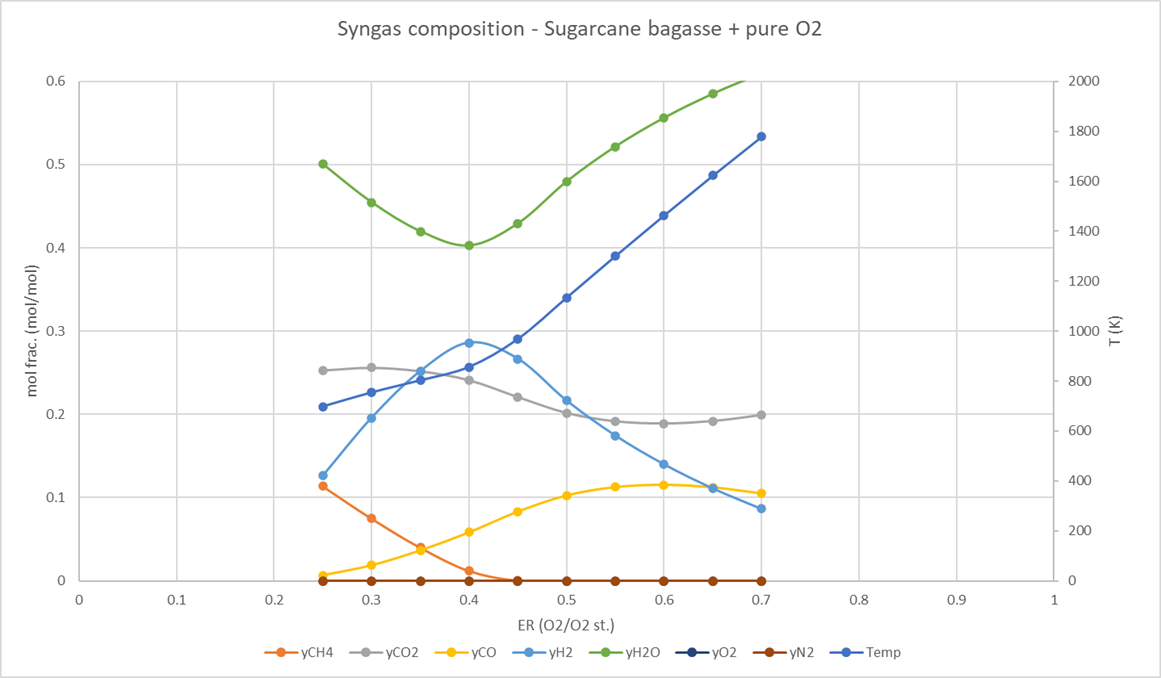
\includegraphics[width=\textwidth]{img/fig_syngasbagacoo2.png}
	\caption{Syngas composition for sugarcane bagasse gasification with pure oxygen}
	\label{img_syngascompO2}
\end{figure}

\begin{figure}
	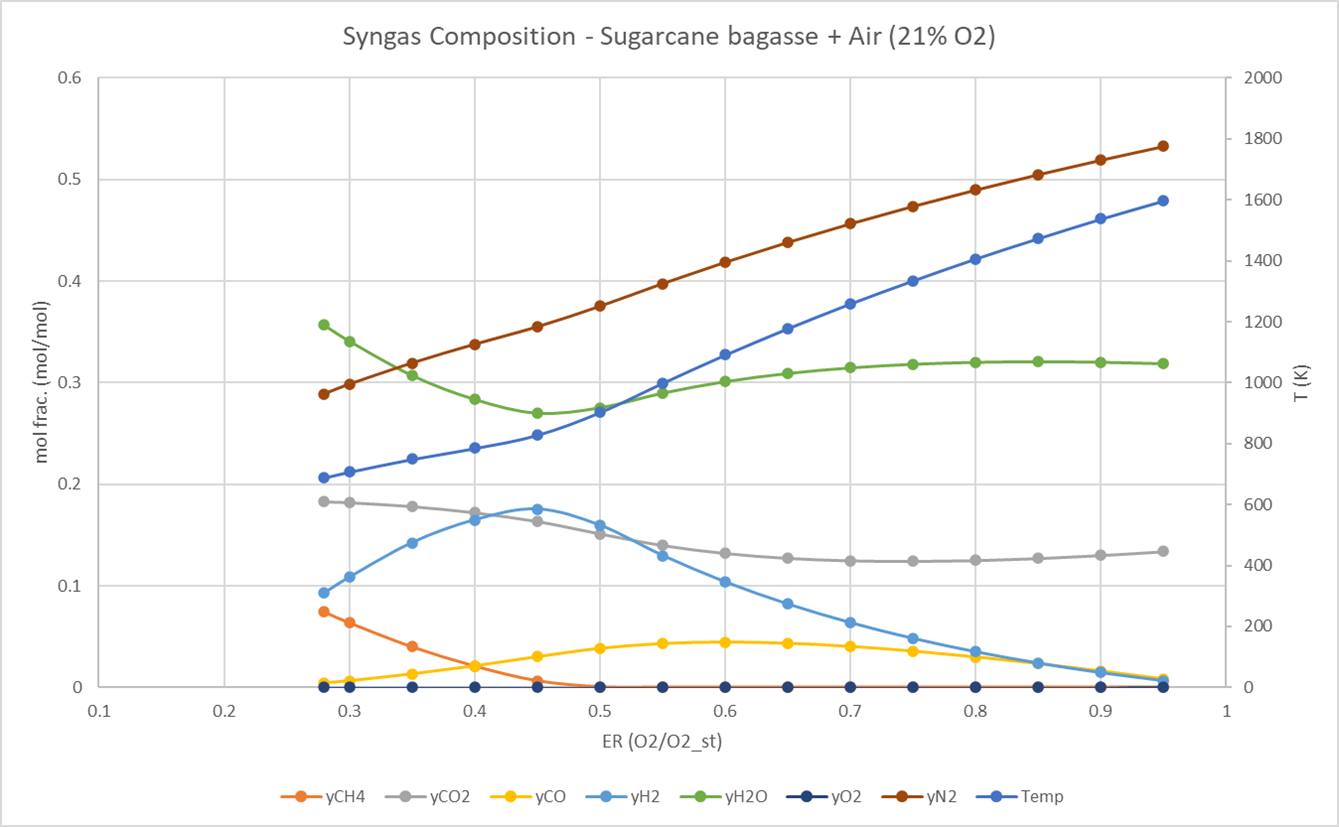
\includegraphics[width=\textwidth]{img/fig_syngasbagacoar.png}
	\caption{Syngas composition for sugarcane bagasse gasification with air}
	\label{img_syngascompair}
\end{figure}

\begin{sidewaystable}
	\caption{Process model main results}
	\small
	\label{tab_mainresults}
	\begin{tabular}{|| c | c | C{0.8cm} | C{0.8cm} | C{0.8cm} | C{0.8cm}| C{0.8cm} | C{0.8cm} |  C{0.8cm} | C{0.8cm}| C{0.8cm} | C{0.8cm} | C{0.8cm} |  C{0.8cm} ||}
		\hline
		Name & Unit & \multicolumn{2}{C{1.6cm} |}{Sugarcane bagasse} & \multicolumn{2}{C{1.8cm} |}{Sugarcane straw} & \multicolumn{2}{C{1.8cm} |}{Soybean straw} & \multicolumn{2}{C{1.8cm} |}{Corn stover} & \multicolumn{2}{C{1.8cm} |}{Rice husk} & \multicolumn{2}{C{1.8cm} |}{Coffee husk} \\
		\hline
		 & & $O_2$ & Air& $O_2$ & Air& $O_2$ & Air& $O_2$ & Air& $O_2$ & Air& $O_2$ & Air \\
		 \hline
		Power generation & kW & 7068 & 8739 & 9412 & 11432 & 10092 & 11047 & 7771 & 9678 & 8791 & 10573 & 9340 & 11293 \\
		Power consumption & kW & 18777 & 18764 & 18672 & 18652 & 24205 & 22628 & 19397 & 19356 & 19399 & 19307 & 22306 & 22546 \\
		Power imports & kW & 11709 & 10025 & 9260 & 7220 & 14113 & 11581 & 11626 & 9678 & 10608 & 8734 & 12966 & 11254 \\
		\hline
		Biomass consumption & kg/h & 62958 & 65768 & 52875 & 55284 & 49812 & 47744 & 43459 & 45262 & 53850 & 55799 & 48338 & 50284 \\
		Biomass consumption & $t_{bio}$/$t_{urea}$ & 1.799 & 1.879 & 1.511 & 1.580 & 1.423 & 1.364 & 1.242 & 1.293 & 1.539 & 1.594 & 1.381 & 1.437 \\
		\hline

		Net power consumption & GJ/$t_{urea}$ & 1.21 & 1.03 & 0.95 & 0.74 & 1.45 & 1.29 & 1.19 & 0.99 & 1.09 & 0.90 & 1.32 & 1.15 \\ 
		Feedstock consumption & GJ/$t_{urea}$ & 20.07 & 20.96 & 20.99 & 21.97 & 20.73 & 21.62 & 20.25 & 21.13 & 22.84 & 23.79 & 20.53 & 21.44 \\
		Total energy consumption & GJ/$t_{urea}$ & 21.49 & 22.17 & 22.11 & 22.84 & 22.43 & 23.15 & 21.65 & 22.30 & 24.12 & 24.85 & 22.08 & 22.79 \\
		\hline
		Levelized cost of urea & USD/$t_{urea}$ & 333.17 & 332.82 & 328.64 & 327.60 & 340.81 & 337.28 & 330.50 & 329.21 & 340.97 & 340.23 & 336.39 & 335.95 \\
		NPV @ 10\% & MMUSD & 119.80 & 120.70 & 131.38 & 134.03 & 100.25 & 109.29 & 126.63 & 129.93 & 99.84 & 101.75 & 111.55 & 112.70 \\
		IRR & \% & 14.53\% & 14.56\% & 14.95\% & 15.05\% & 13.82\% & 14.12\% & 14.78\% & 14.90\% & 13.80\% & 13.87\% & 14.24\% & 14.28\% \\

		Total emissions & kg $CO2_{eq}/t_{urea}$ & 354.70 & 366.65 & 327.83 & 338.43 & - & - & 124.55 & 125.43 & 116.97 & 117.22 & 39.35 & 36.99 \\

		Emission reductions\footnotemark[1] & \% & 86.6\% & 86.1\% & 87.6\% & 87.2\% & - & - & 95.3\% & 95.2\% & 95.6\% & 95.6\% & 98.5\% & 98.6\% \\
	\hline
	\end{tabular}
	\footnotetext[1]{Against 2640 kg CO2 eq / t urea reported for the conventional process}

\end{sidewaystable}

\autoref{tab_mainresults} summarizes the main results. Most of the energy consumption of the plant is in the form of
biomass. The plant is self-sufficient in terms of thermal energy, with a substantial amount of steam being condensed 
at all scenarios.
There is need for power imports from the grid, although net power consumption accounts for about 6\% of the total,
even with large power consumers such as the air separation units and the ammonia compressors. 

The proposed plant achieves an energy consumption between 21.49 and 24.85 GJ/t urea, against 23.34 GJ/t urea for
other published renewable urea plants \cite{zhangTechnoeconomicComparison1002021}. A direct comparison can also be 
made with the traditional process. \autoref{tab_conventionalurea} summarizes the main KPIs for the traditional process.
\textcite{chenPerformanceComparisonUrea2022} evaluated several key performance indicators for multiple types of
traditional fossil fuel urea plants. A traditional fossil fuel urea plant using natural gas as feedstock and 
carbon dioxide stripping achieves an energy consumption of 18.40 GJ/t. While there is room for improvement, 
the plant is already competitive with the traditional process in terms of energy efficiency.

\begin{table}
	\centering
	\caption{Main KPIs for the conventional urea process}
	\label{tab_conventionalurea}
	\begin{tabular}{|| c | c | c||}
		\hline
		Name & Unit & Value \\
		\hline
		Total energy consumption & GJ/$t_{urea}$ & 18.40 \\
		Total emissions & kg $CO2_{eq}/t_{urea}$ & 2640 \\
		\hline
	\end{tabular}
\end{table}

This energy efficiency loss is offset by the large environmental gains of renewable urea. Considering the worst scenario
(processing sugarcane bagasse with air mixed gasification), The proposed plant achieves emissions of 
366.65 kg $kg CO2_{eq} / t_{urea}$, against 2640 $kg CO2_{eq} / t_{urea}$ for the conventional process. These emissions already
consider the full emissions for the life cycle analysis of the sugarcane bagasse 
\cite{jonkerEconomicPerformanceGHG2019}. This accounts for a 86.6\% reduction in emissions, or 2285 $kg CO2_{eq} / t_{urea}$
in emission savings.

The levelized cost of urea was calculated between 327.6 and 340.8 USD / ton, which puts the product at a
competitive cost against current market prices. Using a selling price of USD 380 / t urea, and with a USD 368 
million CAPEX, the plant reaches a maximum NPV of USD 134 million, with an IRR of 15.05\%. These indicators do not take
any kind of carbon tax into account.

Mixed air and oxygen gasification has lower energy efficiencies compared to pure oxygen gasification. However, 
the plant's overall financial performance is marginally improved, since there's a large increase in steam and power
generation with higher air intake on the gasifier. To ensure the gasification autothermal operation, it's still
impossible to completely eliminate the oxygen intake. In scenarios with higher power and lower biomass costs, 
this alternative can become significantly better and vice-versa.

Comparatively, sugarcane bagasse is the best biomass in terms of total energy efficiency, but sugarcane straw presents
the best financial results, given the lower power import required. The power consumption is very sensitive to biomass
composition and moisture, with the best results being presented for biomasses with low moisture and high oxygen content.
Air separation compressors account for about 25\% of the total power consumption, and high oxygen content reduces
the $O_2$ needed on the gasification step.

The following sensitivity analysis considers the first scenario (sugarcane bagasse with pure oxygen gasification)
as the basis of comparison. \autoref{img_IRRsens_carbon} shows the IRR sensitivity to an eventual carbon tax, 
assuming that the emissions savings will enter the plant as a revenue stream.
It is clear that the plant’s financial performance improves significantly in the event of future carbon taxing.

Finally, \autoref{img_IRRsens_capex}, \autoref{img_IRRsens_urea}, \autoref{img_IRRsens_biomass} and
\autoref{img_IRRsens_power} show the IRR sensitivity to the total capital cost, urea price,
biomass price and power price, keeping all other values constant. The plant's profitability is very dependent on
biomass and urea prices, however it is very resilient to power price fluctuations, with good rates of return
even with 60\% higher power prices compared to today's.


\begin{figure}
	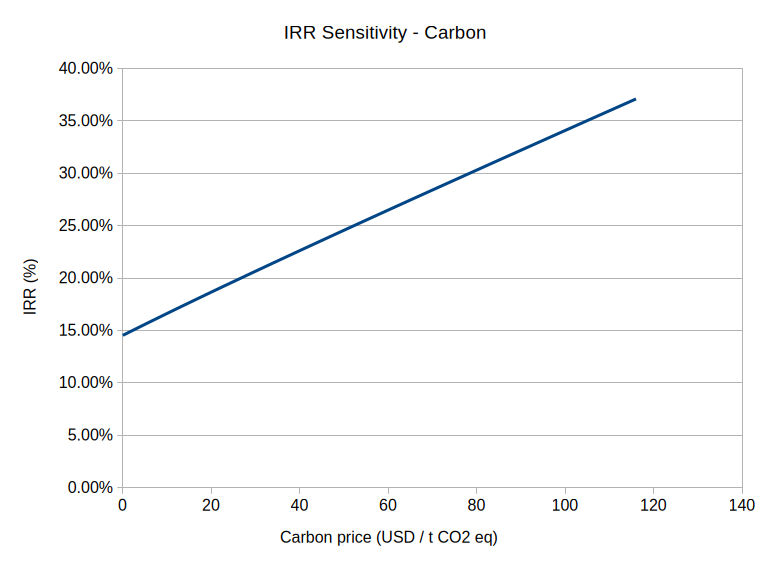
\includegraphics[width=\textwidth]{img/fig_IRRsensitivity_carbon.png}
	\caption{IRR sensitivity to carbon tax}
	\label{img_IRRsens_carbon}
\end{figure}

\begin{figure}
	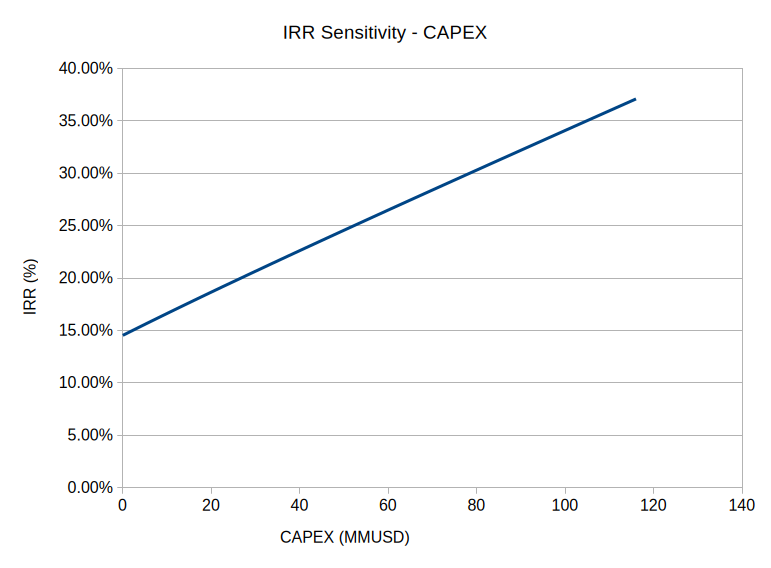
\includegraphics[width=\textwidth]{img/fig_IRRsensitivity_capex.png}
	\caption{IRR sensitivity to CAPEX}
	\label{img_IRRsens_capex}
\end{figure}

\begin{figure}
	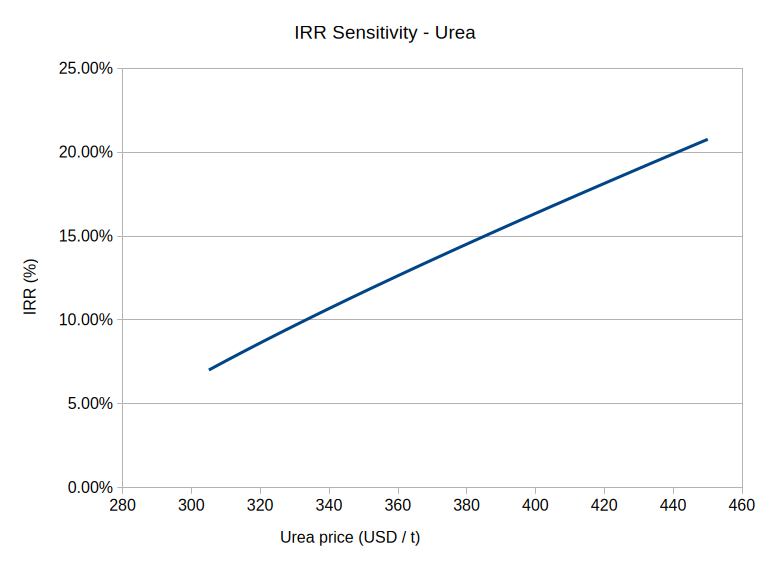
\includegraphics[width=\textwidth]{img/fig_IRRsensitivity_urea.png}
	\caption{IRR sensitivity to urea price}
	\label{img_IRRsens_urea}
\end{figure}


\begin{figure}
	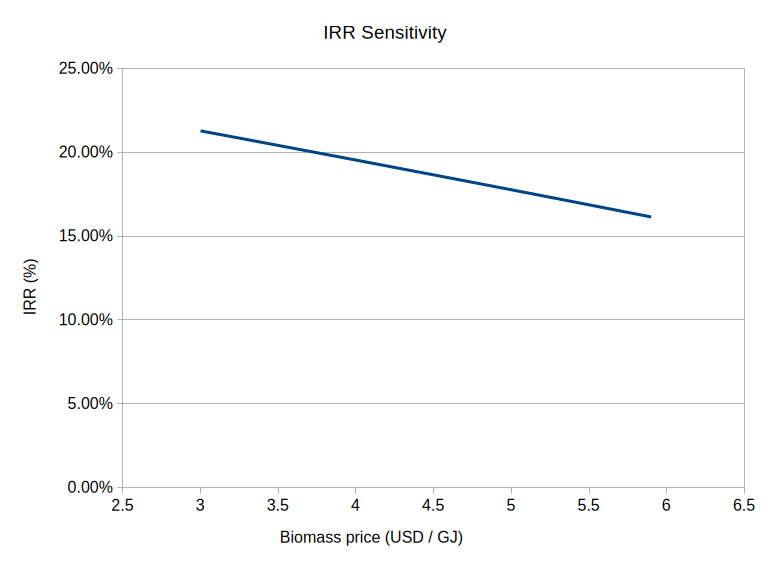
\includegraphics[width=\textwidth]{img/fig_IRRsensitivity_biomass.png}
	\caption{IRR sensitivity to biomass price}
	\label{img_IRRsens_biomass}

\end{figure}


\begin{figure}
	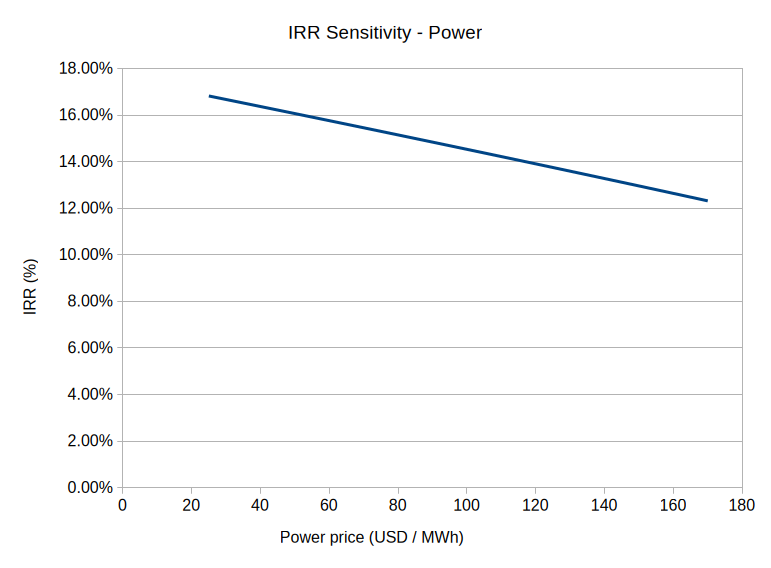
\includegraphics[width=\textwidth]{img/fig_IRRsensitivity_power.png}
	\caption{IRR sensitivity to power price}
	\label{img_IRRsens_power}
\end{figure}

\subsection{Supply-chain model}

The model was applied to several subsets of data, starting with the full dataset at the micro-region level, totaling
558 locations. The commercial solver Gurobi was used to solve the MILP model, taking 19.11 mins on average on a Ryzen 7 CPU at the 
largest simulation. The database used in the simulations, as well as the full results, are provided in the
supplementary material. \autoref{tab_scenarios} provides a description of the scenarios simulated, while 
\autoref{tab_optimizationresults} provides the summary of the results.

The optimization model was initially applied to the whole country at the micro-region level (Scenario 1) In this
scenario, it was found that the Jaboticabal microregion in the state of São Paulo is the optimal location for the installation of the renewable urea plant. Despite being one of the worst performing biomasses in terms of energy efficiency, sugarcane straw was the
optimal biomass, processed via the air mixed gasification route. The optimal region can supply 100\% of the required biomass,
while the close proximity to the large sugarcane crops in the state is beneficial to the urea distribution. 
 \autoref{img_optimizationresults_1} shows the plant location and urea distribution networks.

\begin{table}
	\centering
	\caption{Scenarios simulated in the supply-chain model}
	\label{tab_scenarios}
	\begin{tabular}{||c | c ||}
		Scenario 1 & Whole country at micro-region level \\
		Scenario 2 & Midwest region only \\
		Scenario 3 & South region only \\
		Scenario 4 & Northeast region only \\
		Scenario 5 & North region only \\ 
		Scenario 6 & lower urea demand (25\%) \\ 
		Scenario 7 & Corn stover \\ 
		Scenario 8 & Rice husks \\ 
		Scenario 9 & Coffee husks \\ 
		Scenario 10 & Unconstrained capacity \\ 

	\end{tabular}
\end{table}

\begin{figure}
	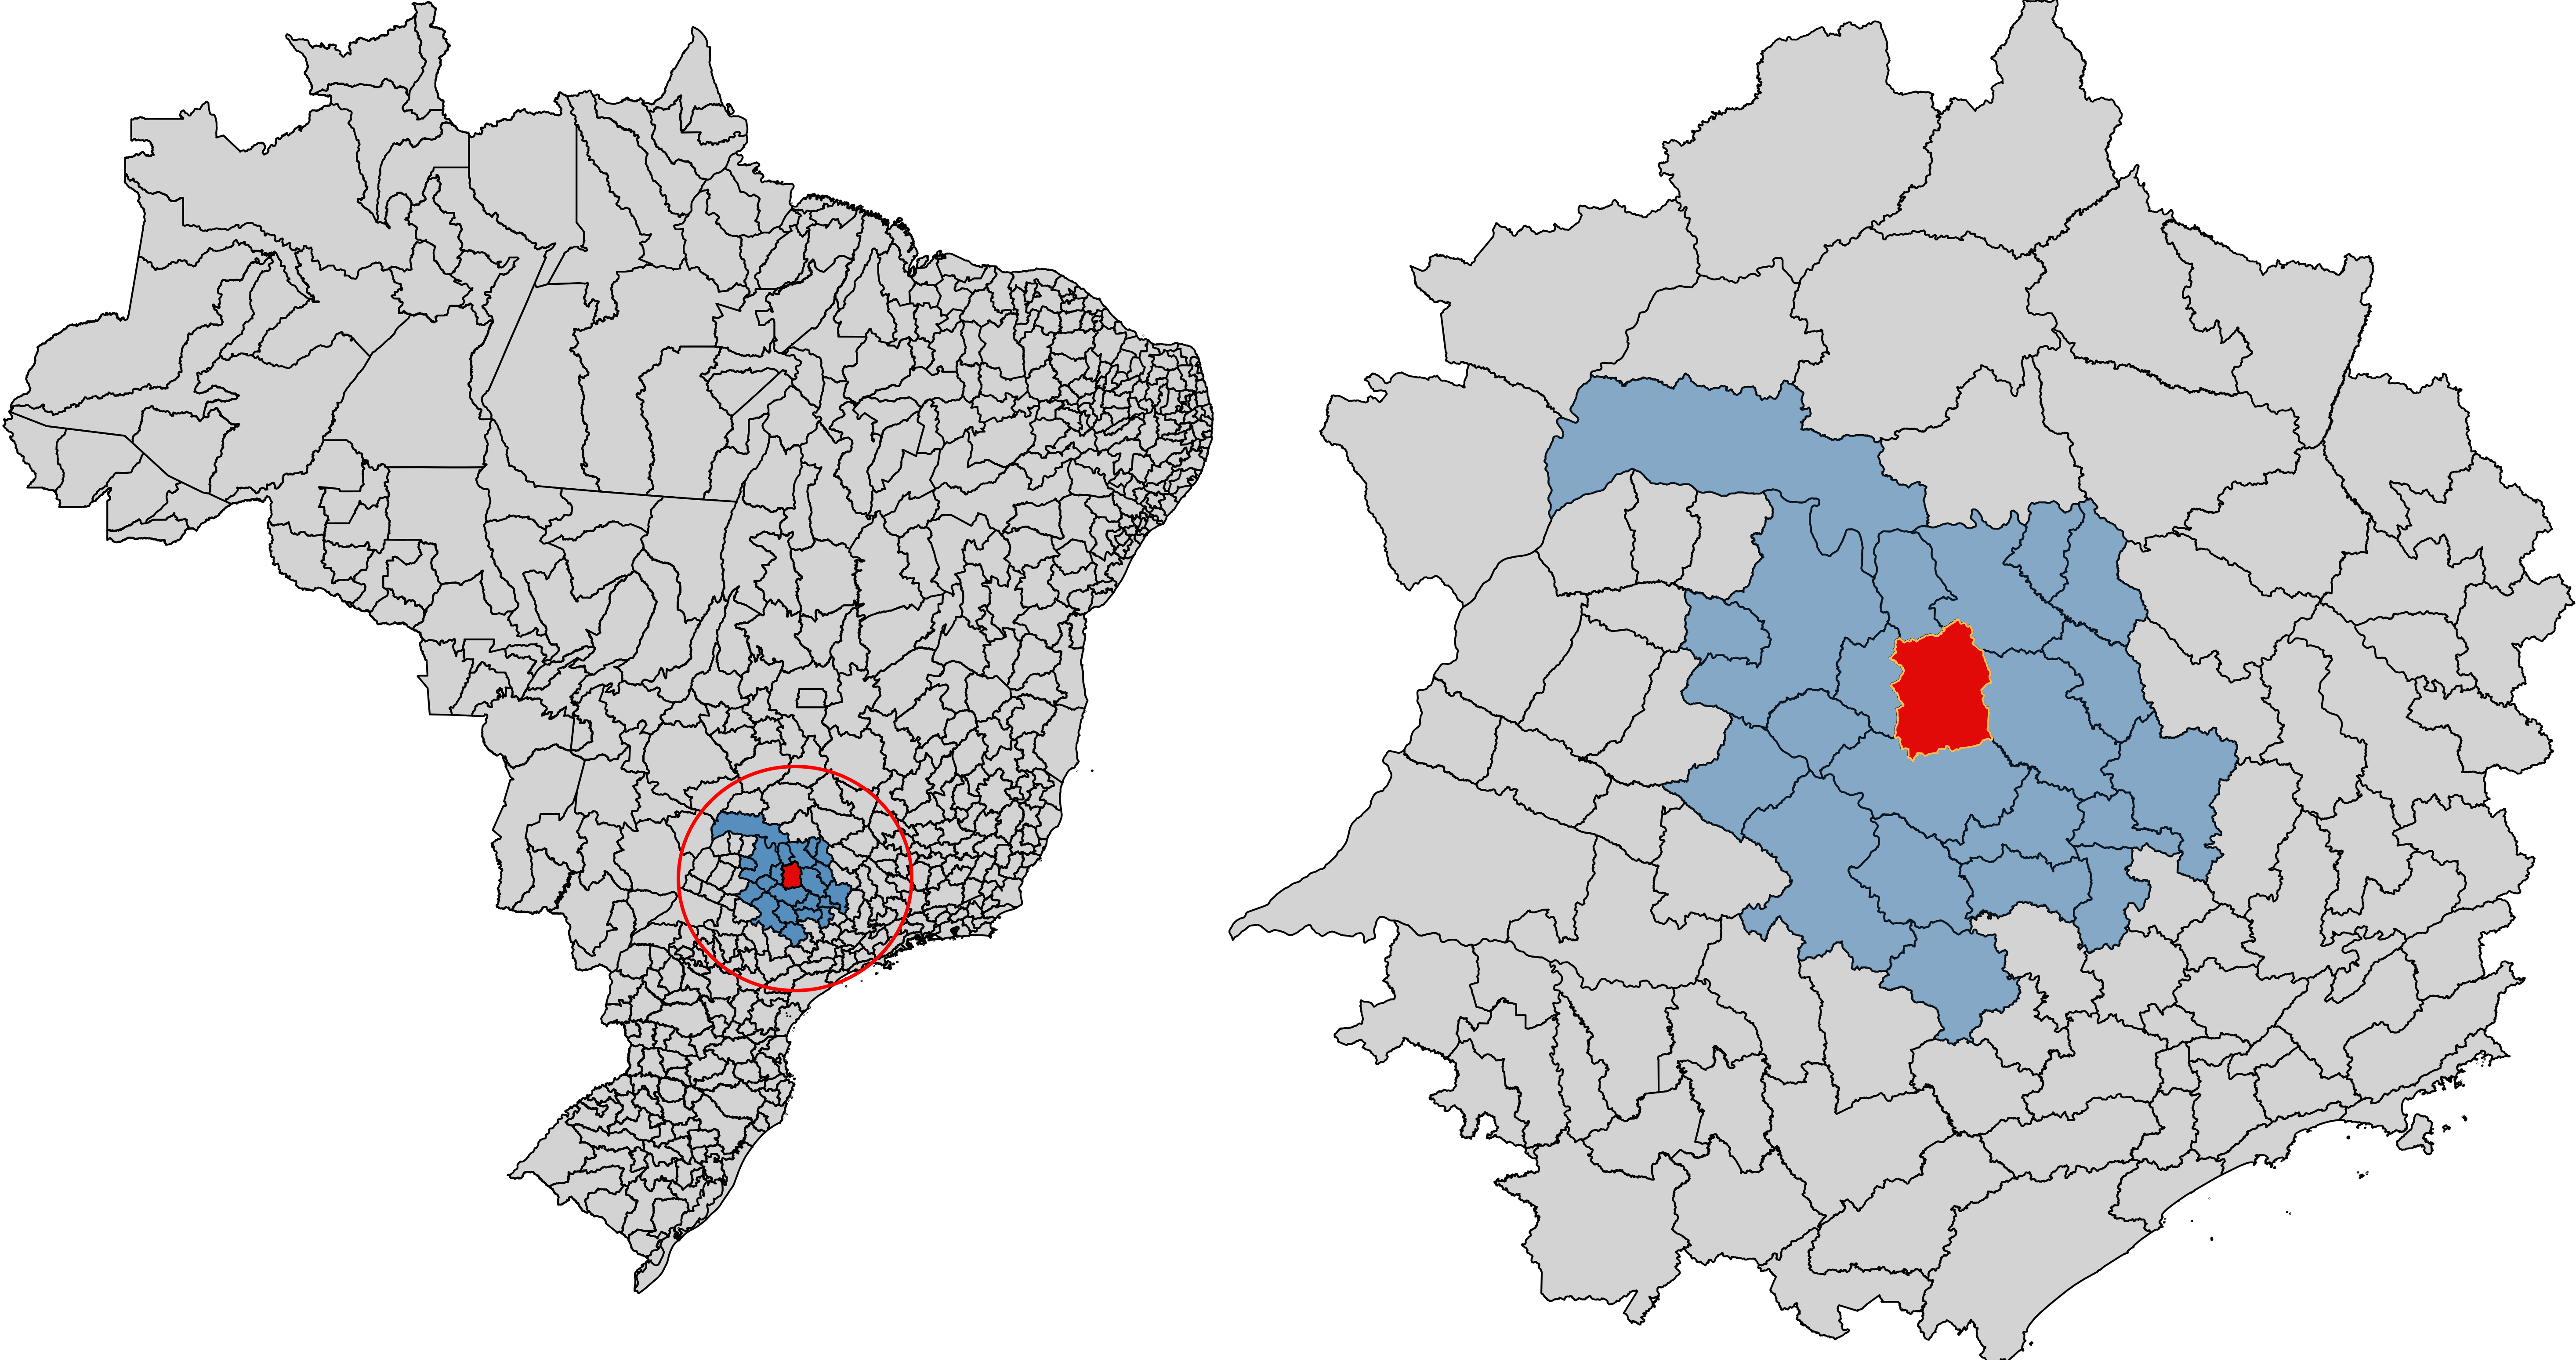
\includegraphics[width=\textwidth]{img/optimization_result_1.png}
	\caption{Optimization model results - Scenario 1. Plant location (red), urea distribution (blue)}
	\label{img_optimizationresults_1}
\end{figure}

Scenarios 2, 3, 4 and 5 were generated constraining the plant location to the Midwest, South, Northeast and North
geographical regions of the country, respectively. The Midwest and South regions show similar feasibility with very close
NPV and LCOU compared to the main scenario, using the same biomass and processing route. The North and Northeast
regions shows the highest LCOU and the smallest capacity of all scenarios. \autoref{img_optimizationresults_4} shows the optimal plant location and urea consumers for scenario 4. As the agricultural density and urea demand per micro-region are lower, the product needs to be distributed across larger distances, increasing logistical costs and affecting the performance of the plant.

\begin{figure}
	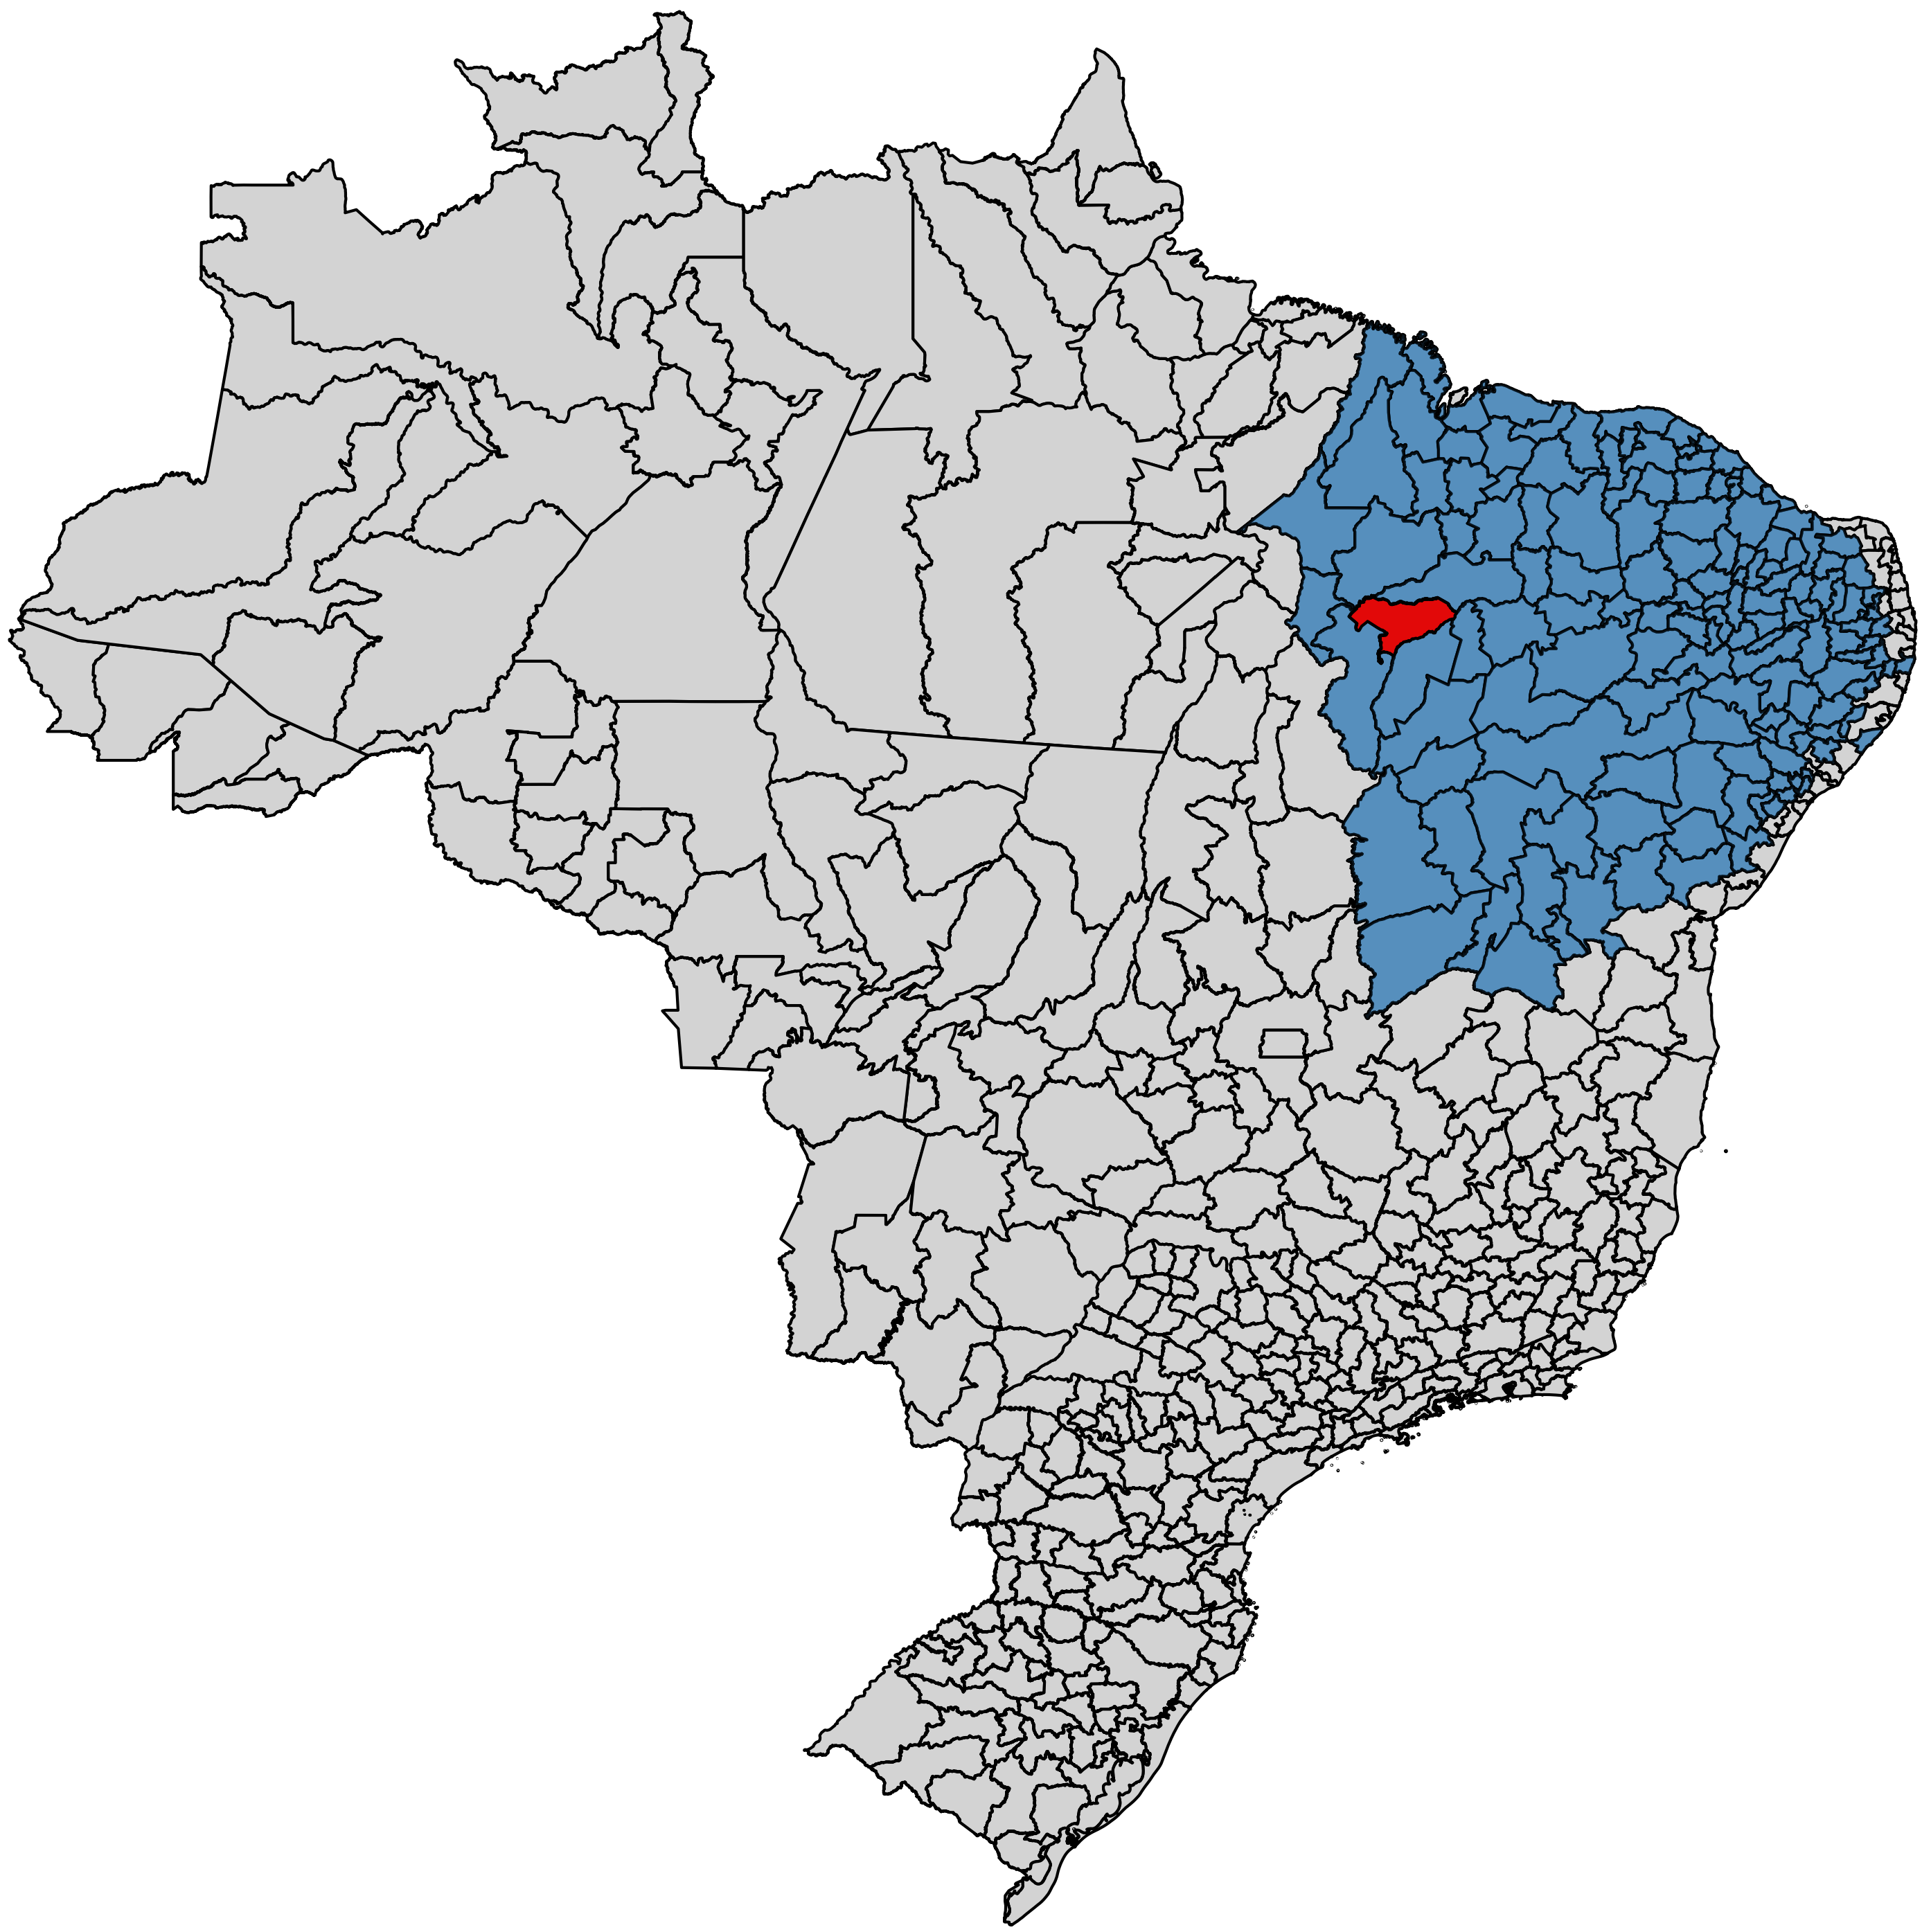
\includegraphics[width=\textwidth]{img/optimization_result_4.png}
	\caption{Optimization result - Scenario 4 - Northeast region only. Plant location (red), urea distribution (blue)}
	\label{img_optimizationresults_4}
\end{figure}

\begin{sidewaystable}
	\caption{Optimization model results}
	\label{tab_optimizationresults}
	\begin{tabular}{|| c | c | c | c  | c | c | c | c | c | c | c | c ||}
		\hline
		 & Unit & 1 & 2 & 3 & 4 & 5 & 6 & 7 & 8 & 9 & 10 \\
		 \hline
		Plant capacity & t/h & 0.0 & 0.0 & 80.0 & 72.8 & 28.0 & 80.0 & 80.0 & 80.0 & 33.5 & 244.9 \\
		Revenue & MMUSD & 260.98 & 260.98 & 260.98 & 237.61 & 91.21 & 260.98 & 260.98 & 260.98 & 109.22 & 798.88 \\
		Biomass costs & MMUSD & 68.07 & 68.07 & 67.75 & 58.48 & 23.65 & 68.07 & 65.54 & 73.35 & 26.85 & 208.37 \\
		Power costs & MMUSD & 14.8 & 14.18 & 14.1 & 19.02 & 5.66 & 14.1 & 18.3 & 16.14 & 10.74 & 45.31 \\
		Transport costs – Biomass & MMUSD & 6.27 & 6.27 & 6.21 & 4.96 & 2.13 & 6.27 & 5.63 & 12.34 & 6.18 & 19.2 \\
		Transport costs – Urea & MMUSD & 8.52 & 11.73 & 11.4 & 28.28 & 8.49 & 18.33 & 11.07 & 18.5 & 4.71 & 58.5 \\
		Fixed costs & MMUSD & 30.89 & 30.89 & 30.89 & 28.32 & 12.18 & 30.89 & 30.89 & 30.89 & 14.19 & 90.12 \\
		Total costs & MMUSD & 128.55 & 131.15 & 130.35 & 139.04 & 52.11 & 137.67 & 131.44 & 151.23 & 62.67 & 421.49 \\
		FCF & MMUSD & 132.43 & 129.83 & 130.64 & 98.56 & 39.1 & 123.32 & 129.54 & 109.76 & 46.54 & 377.39 \\
		NPV & MMUSD & 355.17 & 333.05 & 339.9 & 131.19 & 28.41 & 277.57 & 330.58 & 162.14 & 41.43 & 959.99 \\
		LCOU & USD / t urea & 319.3 & 323 & 321.9 & 355.4 & 366.1 & 332.5 & 323.5 & 352.3 & 363.1 & 326.4 \\
		CAPEX & MMUSD & 772.29 & 772.29 & 772.29 & 707.94 & 304.50 & 772.30 & 772.30 & 772.30 & 354.83 & 2252.90 \\
		\hline
	\end{tabular}

\end{sidewaystable}

Scenario 6 considers the urea demand to be 25\% of the originally estimated, to account for competition with other
players and external markets. In this scenario, the optimal region shifts to the Presidente Prudente micro-region. While
this region is geographically close to the scenario 1 optimal location, it is better positioned to distribute urea
to a wider number of regions in the country's interior. The plant is still feasible at the maximum capacity of 80 t/h,
however the NPV of the plant is reduced to 277.6 MMUSD, considering the higher urea distribution costs. \autoref{img_optimizationresults_6} illustrates the impact of the lower urea demand on the distribution network size.

\begin{figure}
	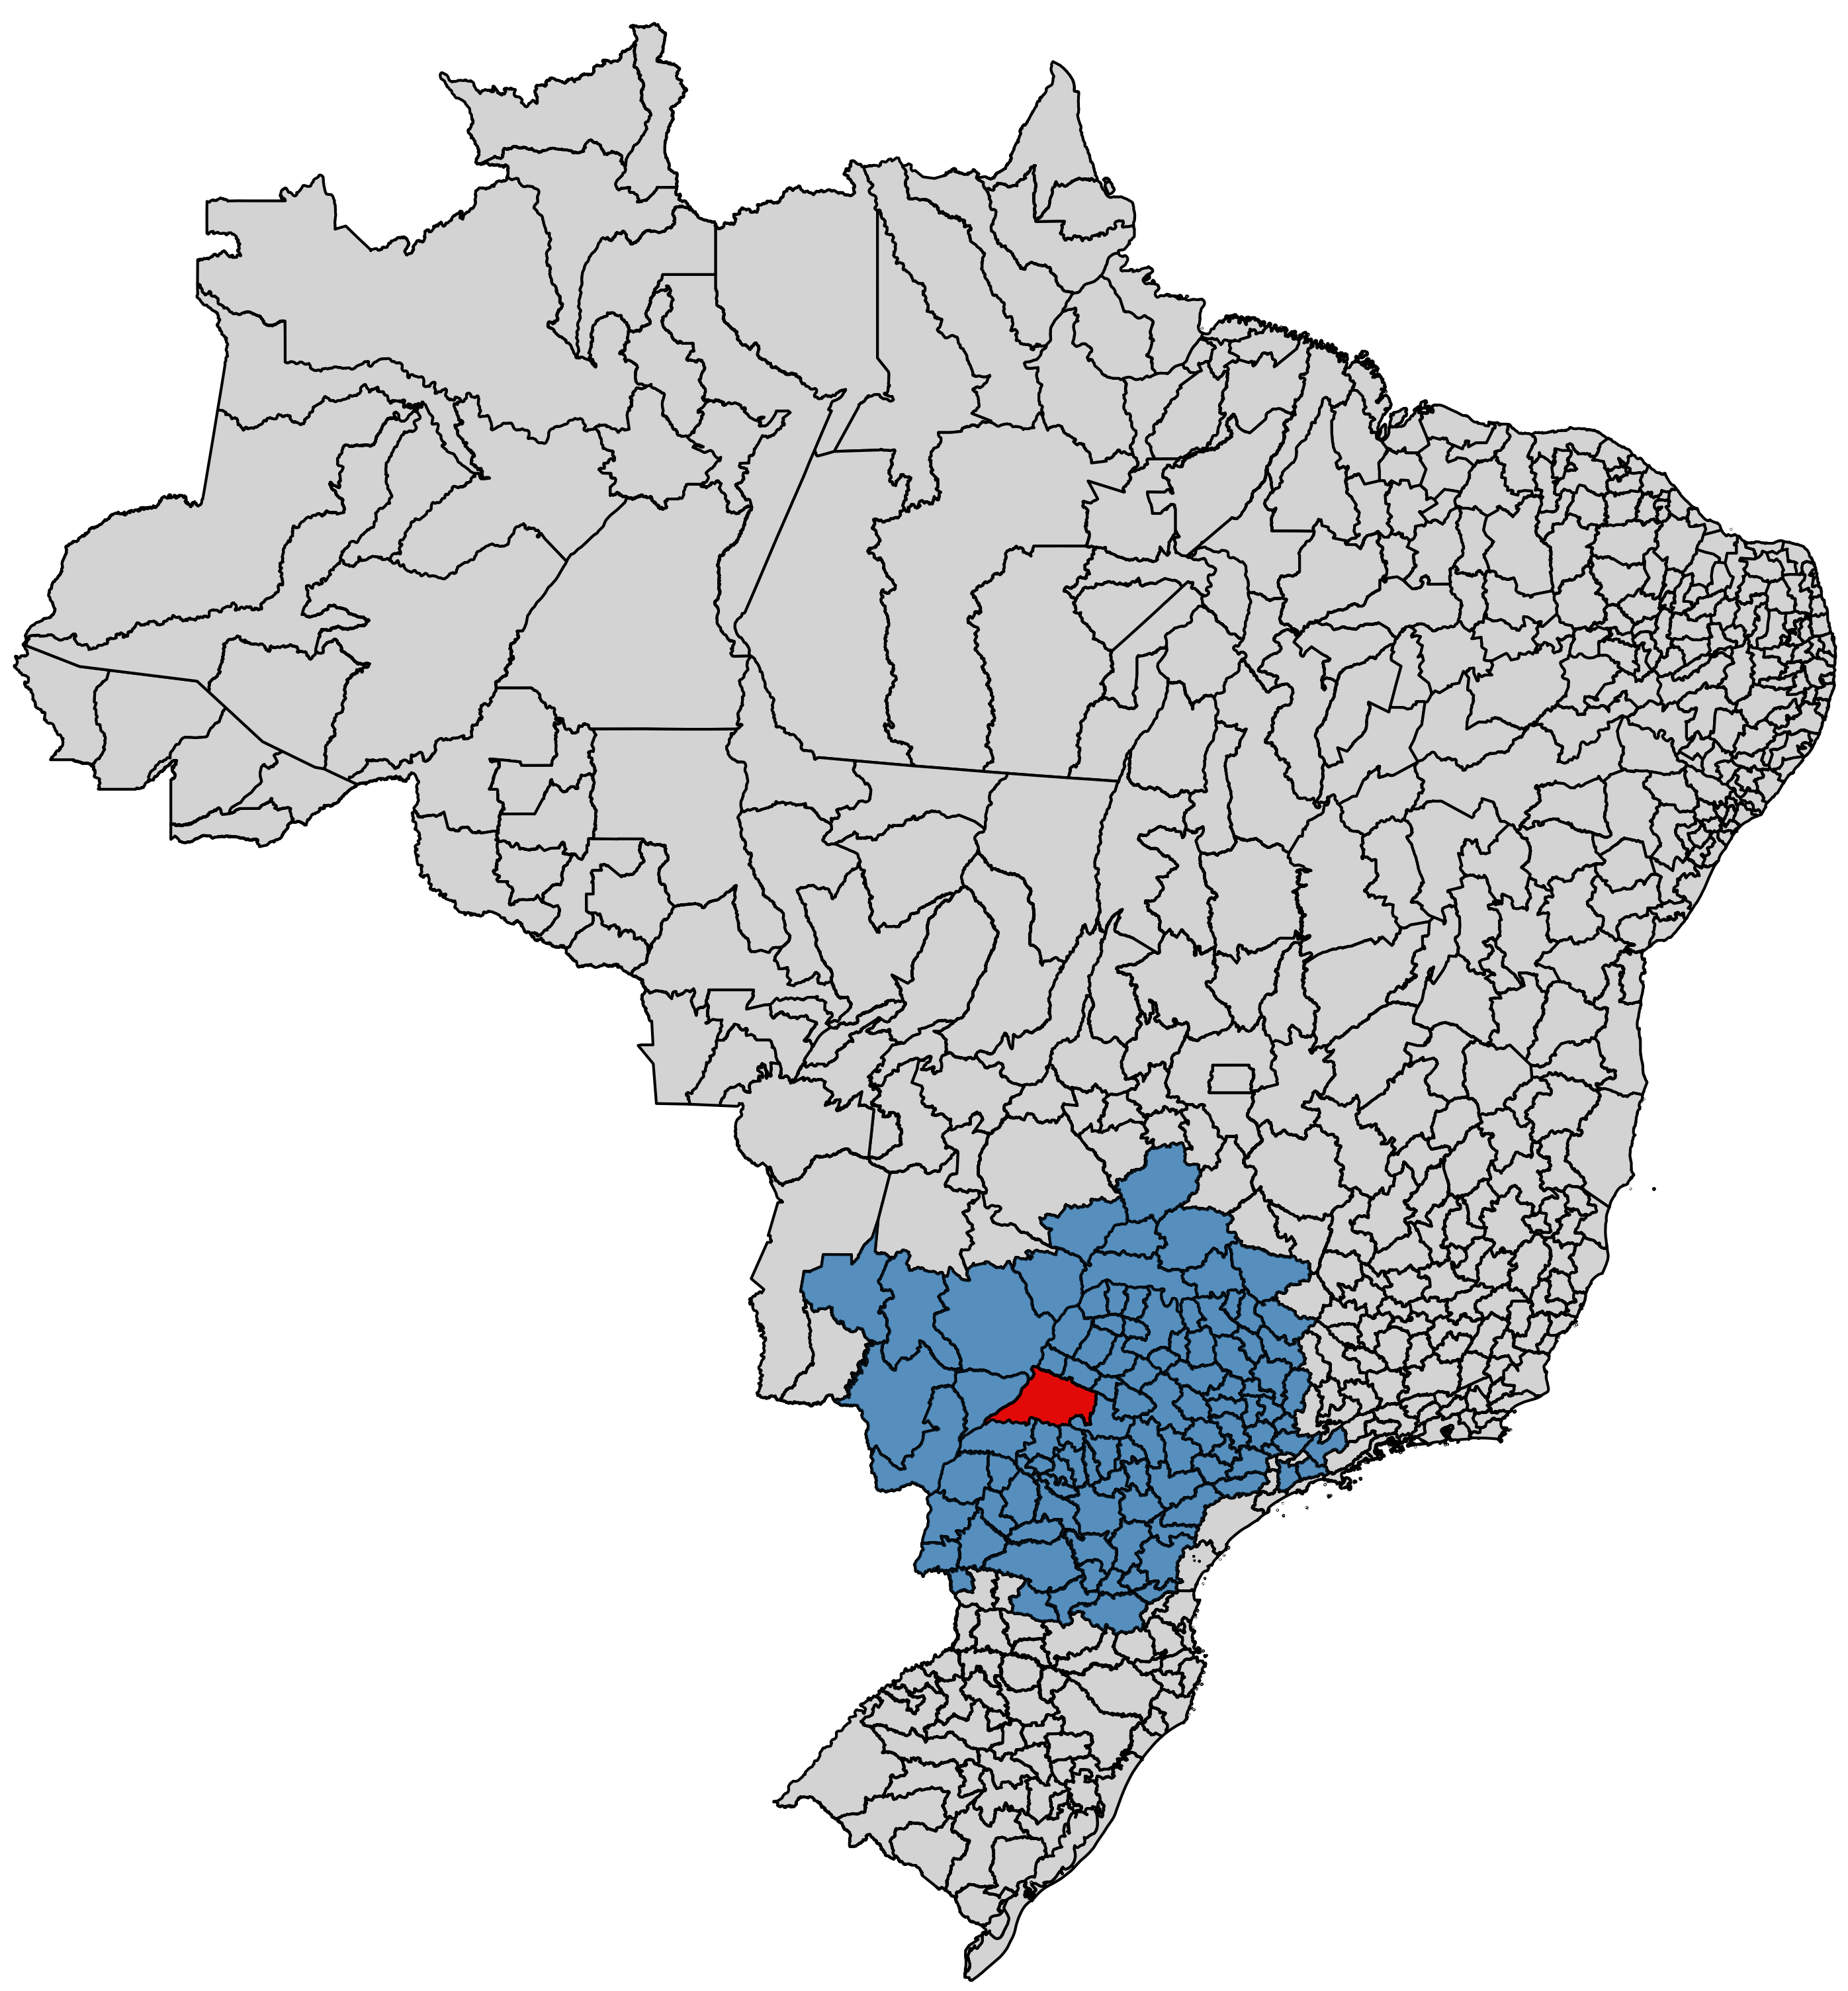
\includegraphics[width=\textwidth]{img/optimization_result_6.png}
	\caption{Optimization result - Scenario 6 - Lower urea demand. Plant location (red), urea distribution (blue)}
	\label{img_optimizationresults_6}
\end{figure}

Additional scenarios were simulated by constraining the feedstock to a single type of residue, other than sugarcane.
Scenario 7 considers that corn stover is the only possible biomass. The plant's profitability is similar to the main scenario,
but the plant location shifts to the Campo Mourão microregion on the Paraná state. 

Scenario 8 considers that rice husk is the only processed biomass. \autoref{img_optimizationresults_8} shows the plant
location, urea and biomass distribution networks. The profitability of the plant is affected by the 
higher power costs of the rice-producing regions and the higher distribution costs of biomass transport at this location,
as the rice husk supply is fragmented in various regions instead of concentrated in a small area.

\begin{figure}
	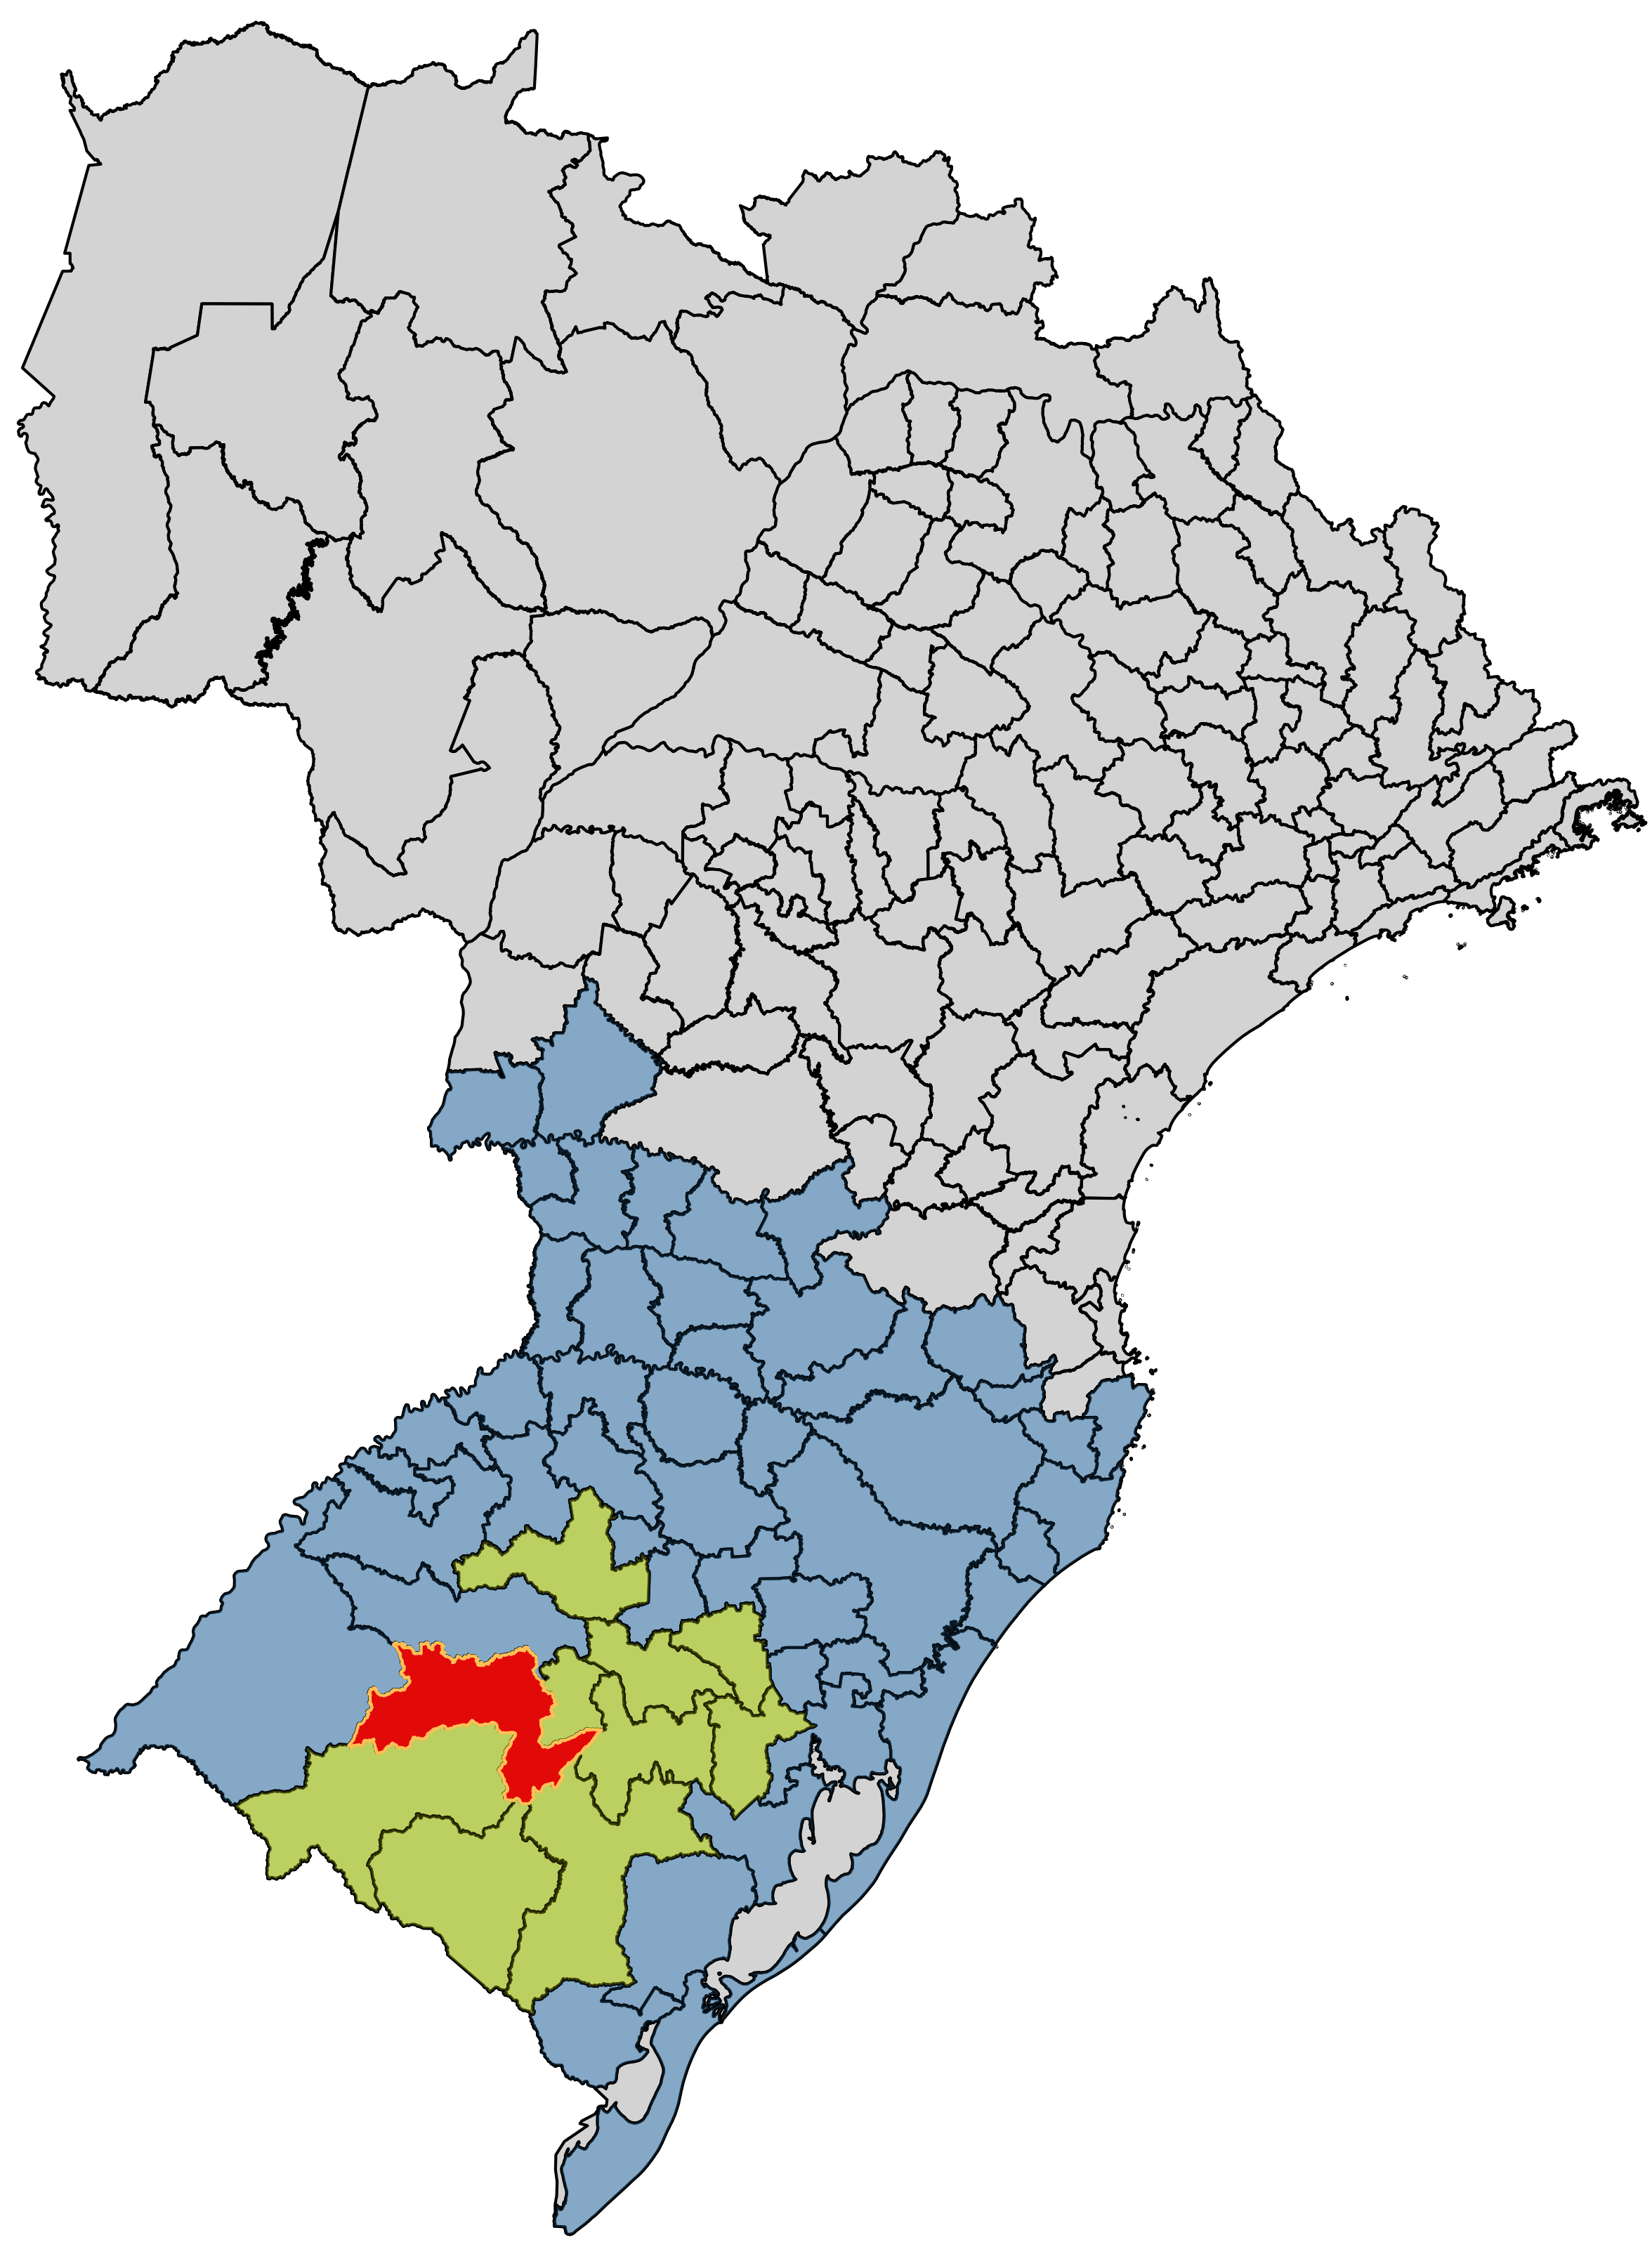
\includegraphics[width=\textwidth]{img/optimization_result_8.png}
	\caption{Optimization result - Scenario 8 - Rice husks only. Plant location (red), urea distribution (blue), biomass distribution (green)}
	\label{img_optimizationresults_8}
\end{figure}

Scenario 9 constrains the biomass to coffee husks. \autoref{img_optimizationresults_9} shows the plant
location, urea and biomass distribution networks. Despite the high urea demand of the coffee production and the good
energy efficiency of the plant processing this biomass, the low biomass generation per kg of coffee and the distributed
nature of this crop's production negatively affects the economic performance of the plant and the optimal plant capacity
, with the biomass having to travel large distances to reach the plant.

\begin{figure}
	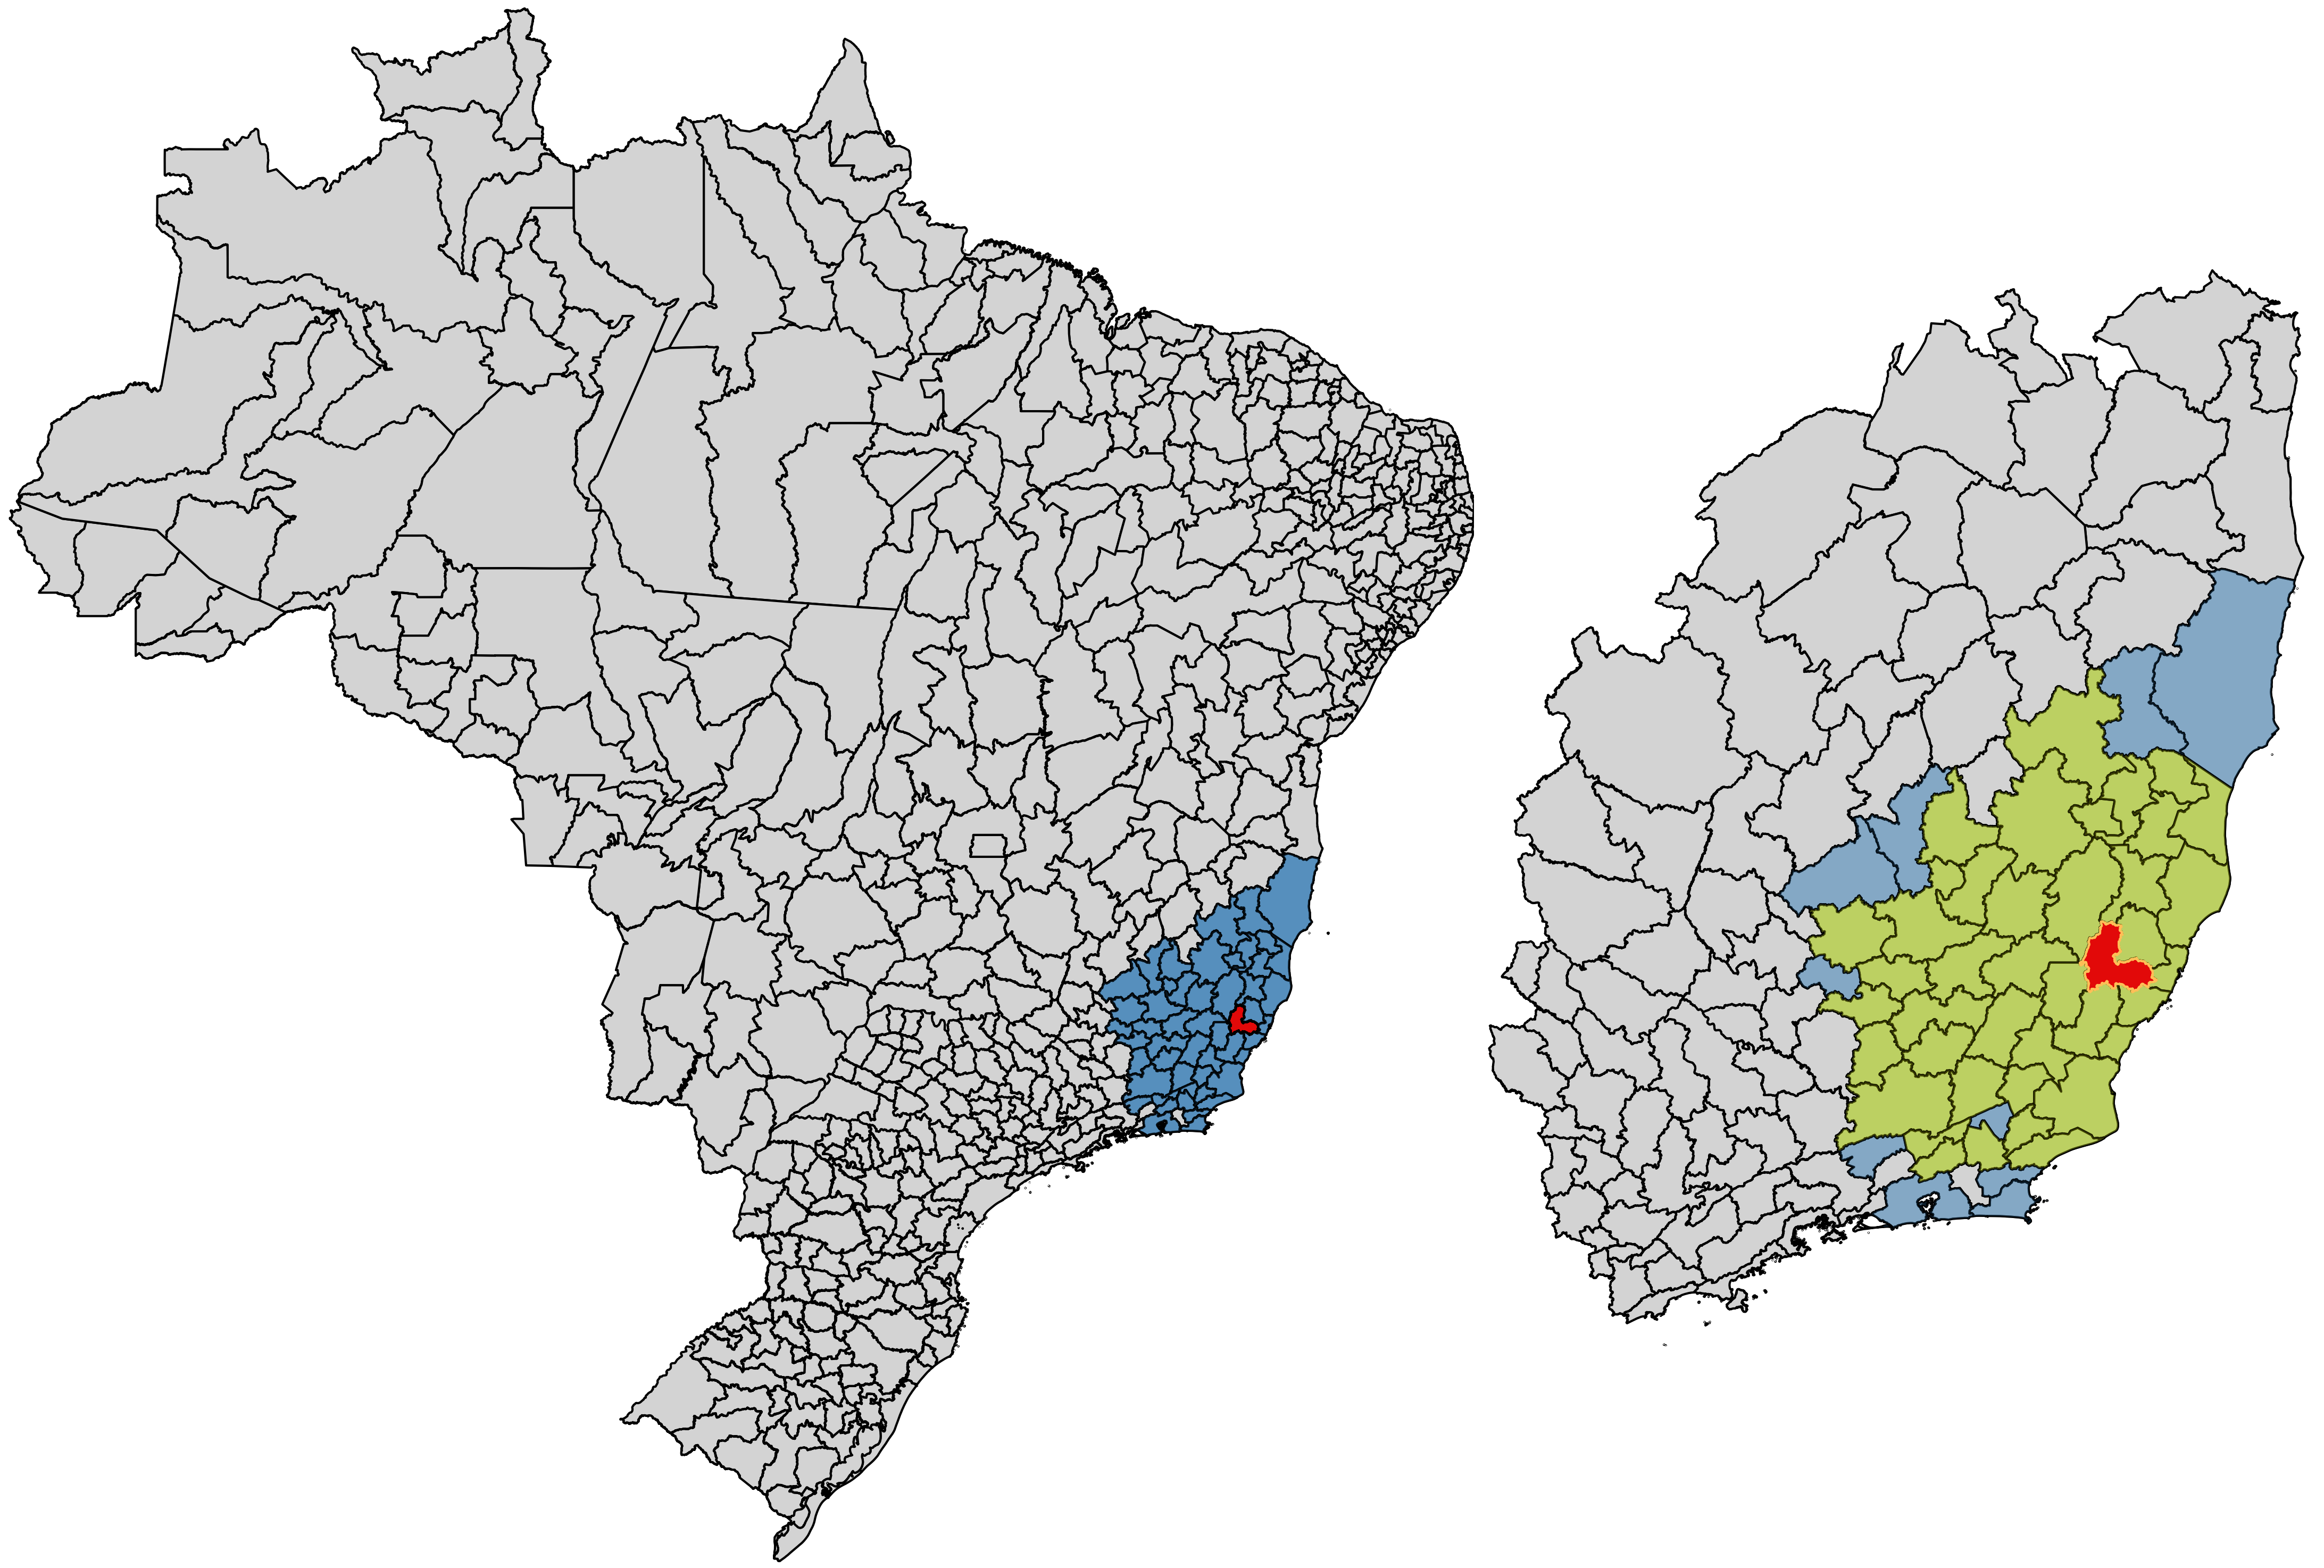
\includegraphics[width=\textwidth]{img/optimization_result_9.png}
	\caption{Optimization result - Scenario 9 - Rice husks only. Plant location (red), urea distribution (blue), biomass distribution (green)}
	\label{img_optimizationresults_9}
\end{figure}


The plant capacity was constrained to a maximum of 80 t/h at the main scenarios. A last scenario with unconstrained
capacity and limited to the Southeast Region was modeled. In this scenario, the optimal region is the Ribeirão Preto one,
with an optimal capacity calculated by the model of 244.9 t/h. Despite the feasibility of this configuration, this capacity
was deemed to large as it accounts for about 25\% of the national urea demand.

\subsection{Conclusions}

A process model for biomass gasification and renewable urea production plant was developed, and its key performance
indicators presented for multiple scenarios of biomass types and operating conditions. It was found that the renewable
urea plant has a lower energy efficiency than the regular fossil fuel route, however the lower prices of biomass compensate
for this efficiency loss to the point where the renewable urea can commercialize with competitive prices, even without
carbon taxation. Environmentally, the renewable urea plant can reduce emissions allocated to urea in about 86.6\%, or
2285 kg $CO2_{eq}$ / ton of urea, already taking into account the life cycle emissions of the biomass. A sensitivity
analysis for the internal rate of return was presented for all the main financial factors such as capital costs,
biomass, urea and power prices. Future carbon taxation was also considered and can improve the financial results
significantly.

The process model results were used in a supply chain optimization model to evaluate the ideal location and plant
configuration considering biomass supply and urea demand constraints. Despite not being the best biomass in terms
of energy efficiency, processing sugarcane straw with air mixed gasification proved to be the ideal operational scenario
for the plant. Multiple scenarios were simulated in different regions of the country and limiting the feedstock to distinct biomasses. Overall, the distribution of urea proved to be the critical factor in the feasibility of the plant. This highlights
the need for a robust supply chain model coupled with a traditional process modeling approach.

\clearpage

\printbibliography{}

\end{document}
